%%%%%%%%%%%%%%%%%%%%%%%%%%%%%%%%%%%%%%%%%%%%%%%%%%%%%%%%%%%
%%%%%%%%%%%%%%%%%%%%%%%%%%%%%%%%%%%%%%%%%%%%%%%%%%%%%%%%%%%
\section{Parameter Identification and the MUD Point}
%%%%%%%%%%%%%%%%%%%%%%%%%%%%%%%%%%%%%%%%%%%%%%%%%%%%%%%%%%%
%%%%%%%%%%%%%%%%%%%%%%%%%%%%%%%%%%%%%%%%%%%%%%%%%%%%%%%%%%%

%%%%%%%%%%%%%%%%%%%%%%%%%%%%%%%%%%%%%%%%%%%%%%%%%%%%%%%%%%%
\begin{frame}{\it The one where we define the Maximal Updated Density (MUD) point.}

\begin{equation}\label{eq:mudpt_inital_defn}
	\mudpt := \argmax {\updated}(\param)
\end{equation}

\end{frame}

\begin{frame}[t]{\it The one where we create a unifying framework.}

\begin{itemize}
  \item Recall $\norm{\mathbf{x}}_C^2 := (\mathbf{x}, \mathbf{x})_C = \mathbf{x}^T C \mathbf{x}$. \\

  \bigskip
  \item Non-degenerative $\predictedCov^{-1}$, $\observedCov^{-1}$, $\initialCov^{-1}$ play the role of $C$. \\

  \bigskip
  \bigskip
  \item Suppose that $\initial = \prior \sim \mathcal{N}(\param_0, \initialCov)$.

  \bigskip
  \item Suppose $\qoi$ is linear and that $\observed = \pi_\text{like} \sim \mathcal{N}(\observedMean, \observedCov)$.

  \bigskip
  \bigskip
  \item Linearity of $\qoi$ implies that $Q(\param)=A\param$ for some $A\in\RR^{d\times p}$, and that $\predicted \sim \mathcal{N}(Q(\param_0), \predictedCov)$, where

  \begin{equation}\label{eq:predictCov}
  	\predictedCov := A\initialCov A^\top.
  \end{equation}

\end{itemize}


\end{frame}

%%%%%%%%%%%%%%%%%%%%%%%%%%%%%%%%%%%%%%%%%%%%%%%%%%%%%%%%%%
\subsection{Theory of Regularization}
%%%%%%%%%%%%%%%%%%%%%%%%%%%%%%%%%%%%%%%%%%%%%%%%%%%%%%%%%%

\begin{frame}{\it The one with the regularization equations.}

\begin{table}[htbp]
\centering
\begin{equation*}
\begin{split}
\posterior(\param\,|\,d) &= \frac{\prior(\param)\pi_\text{like}(d\,|\,\param)}{\int_{\pspace} \pi_\text{like}(d\, |\, \param)  \prior(\param) d\pmeas} \\
& \\
\updated(\param) &= \initial(\param) \frac{\observed(Q(\param))}{\predicted(Q(\param))}
\end{split}
\end{equation*}

\bigskip
\begin{tabular}{|c|c|}
\hline
& \\
  Tikhonov & $T(\param):=\norm{Q(\param)-\observedMean}_{\observedCov^{-1}}^2 +
      \norm{\param-\initialMean}_{\initialCov^{-1}}^2$ \\
& \\
\hline & \\
  Data-Consistent & $J(\param):=T(\param) - \norm{Q(\param)-Q(\initialMean)}_{\predictedCov^{-1}}^2$ \\
& \\
  \hline
\end{tabular}
% \caption{The $\param$ which minimizes these functionals also maximizes the updated PDF (left) and the Bayesian posterior PDF (right).
%
% $T(\param)$ is the typical functional often associated with Tikhonov regularization.
%
% The $J(\param)$ has an additional term subtracted from $T(\param)$ coming from the predicted density that serves as ``unregularization'' in data--informed directions.}
  \label{tab:func_comparisons}
\end{table}


\end{frame}



%%%%%%%%%%%%%%%%%%%%%%%%%%%%%%%%%%%%%%%%%%%%%%%%%%%%%%%%%%%
\subsection{Linear Example}
%%%%%%%%%%%%%%%%%%%%%%%%%%%%%%%%%%%%%%%%%%%%%%%%%%%%%%%%%%%

%%%%%%%%%%%%%%%%%%%%%%%%%%%%%%%%%%%%%%%%%%%%%%%%%%%%%%%%%%%
\begin{frame}{\it The one where an example highlights a key difference.}

\begin{itemize}
\item $A=\mat{cc}{1 & 1}$

\bigskip
\item 2-D input, 1-D output $\implies$ rank-deficient

\bigskip
\item Details:

\begin{equation*}
\begin{split}
	\initialMean = \mat{cc}{0.25 & 0.25}^\top \\ \\
  \initialCov = \mat{cc}{1 & -0.25 \\ -0.25 & 0.5} \\ \\
  \observedMean=1, \text{ and } \observedCov = \mat{c}{0.25}
\end{split}
\end{equation*}

\end{itemize}
\end{frame}

%%%%%%%%%%%%%%%%%%%%%%%%%%%%%%%%%%%%%%%%%%%%%%%%%%%%%%%%%%%
\begin{frame}{\it The one that kind of says it all.}
%\vskip 25pt
\centering
\begin{figure}
\centering

\begin{figure}
   % 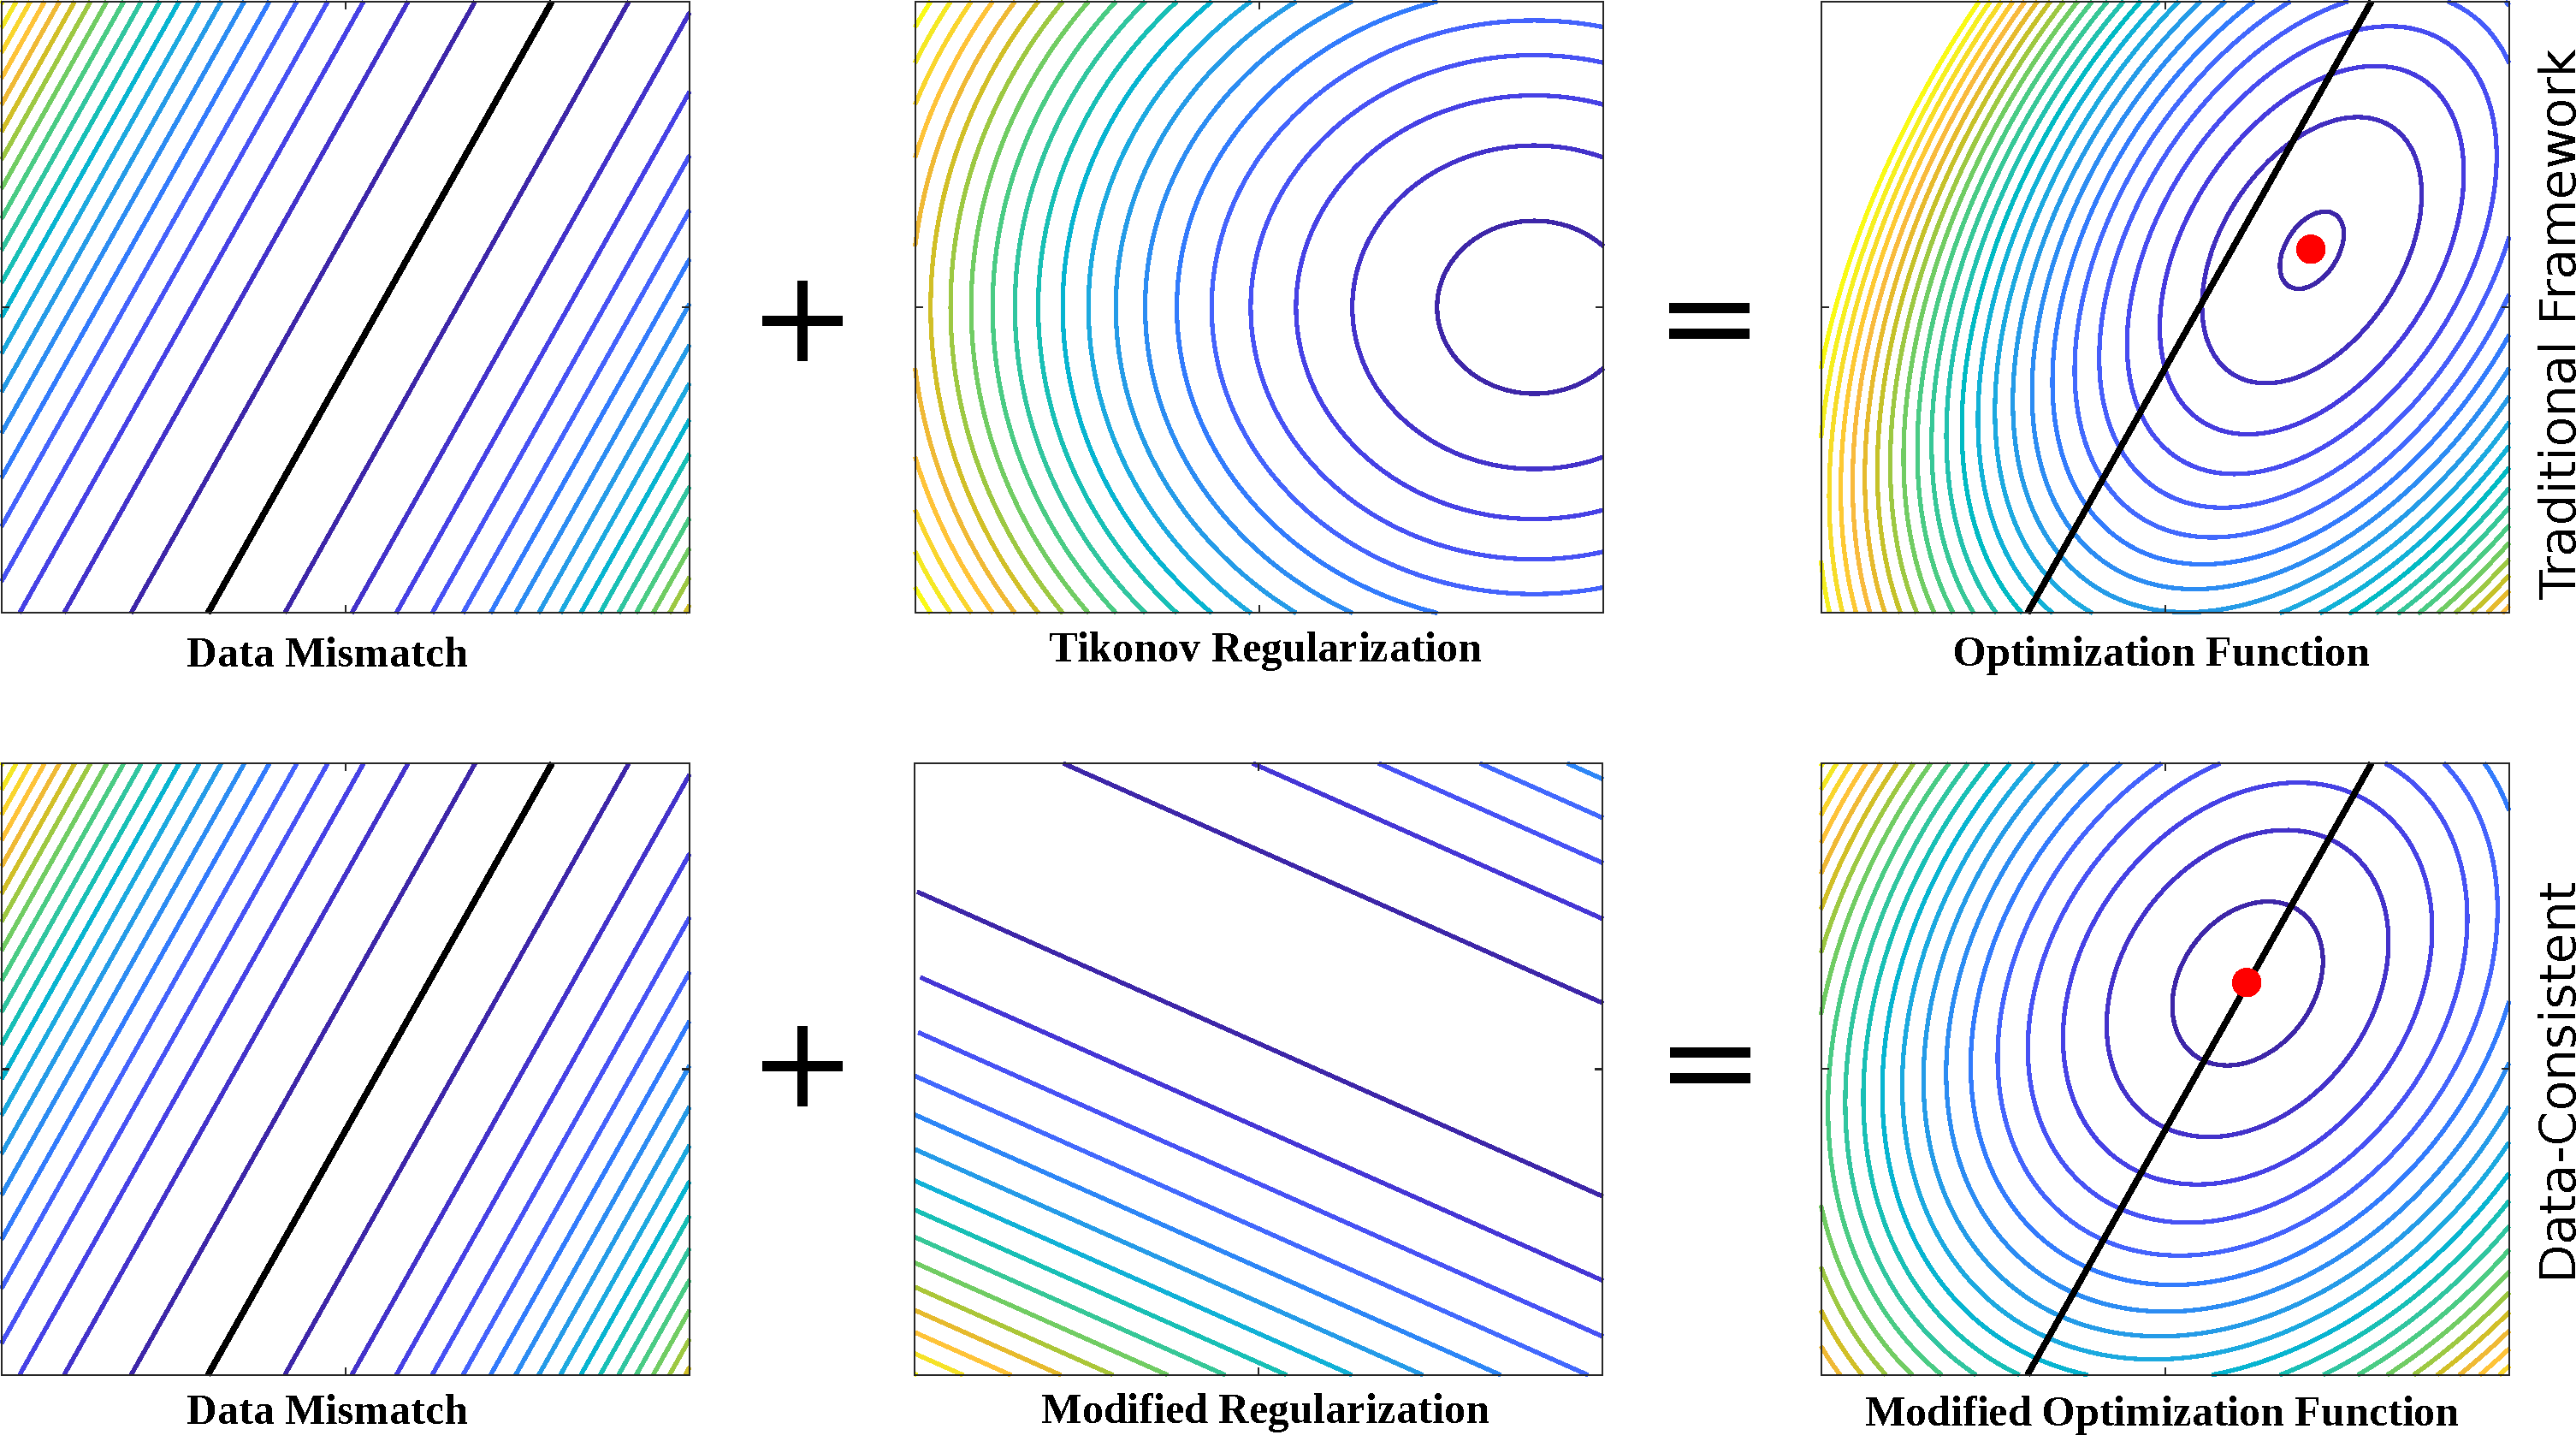
\includegraphics[width=\linewidth]{figures/Regularization-all-in-one.pdf}
  \centering
  \begin{tabular}{|ccc|}
    \hline
      \subf{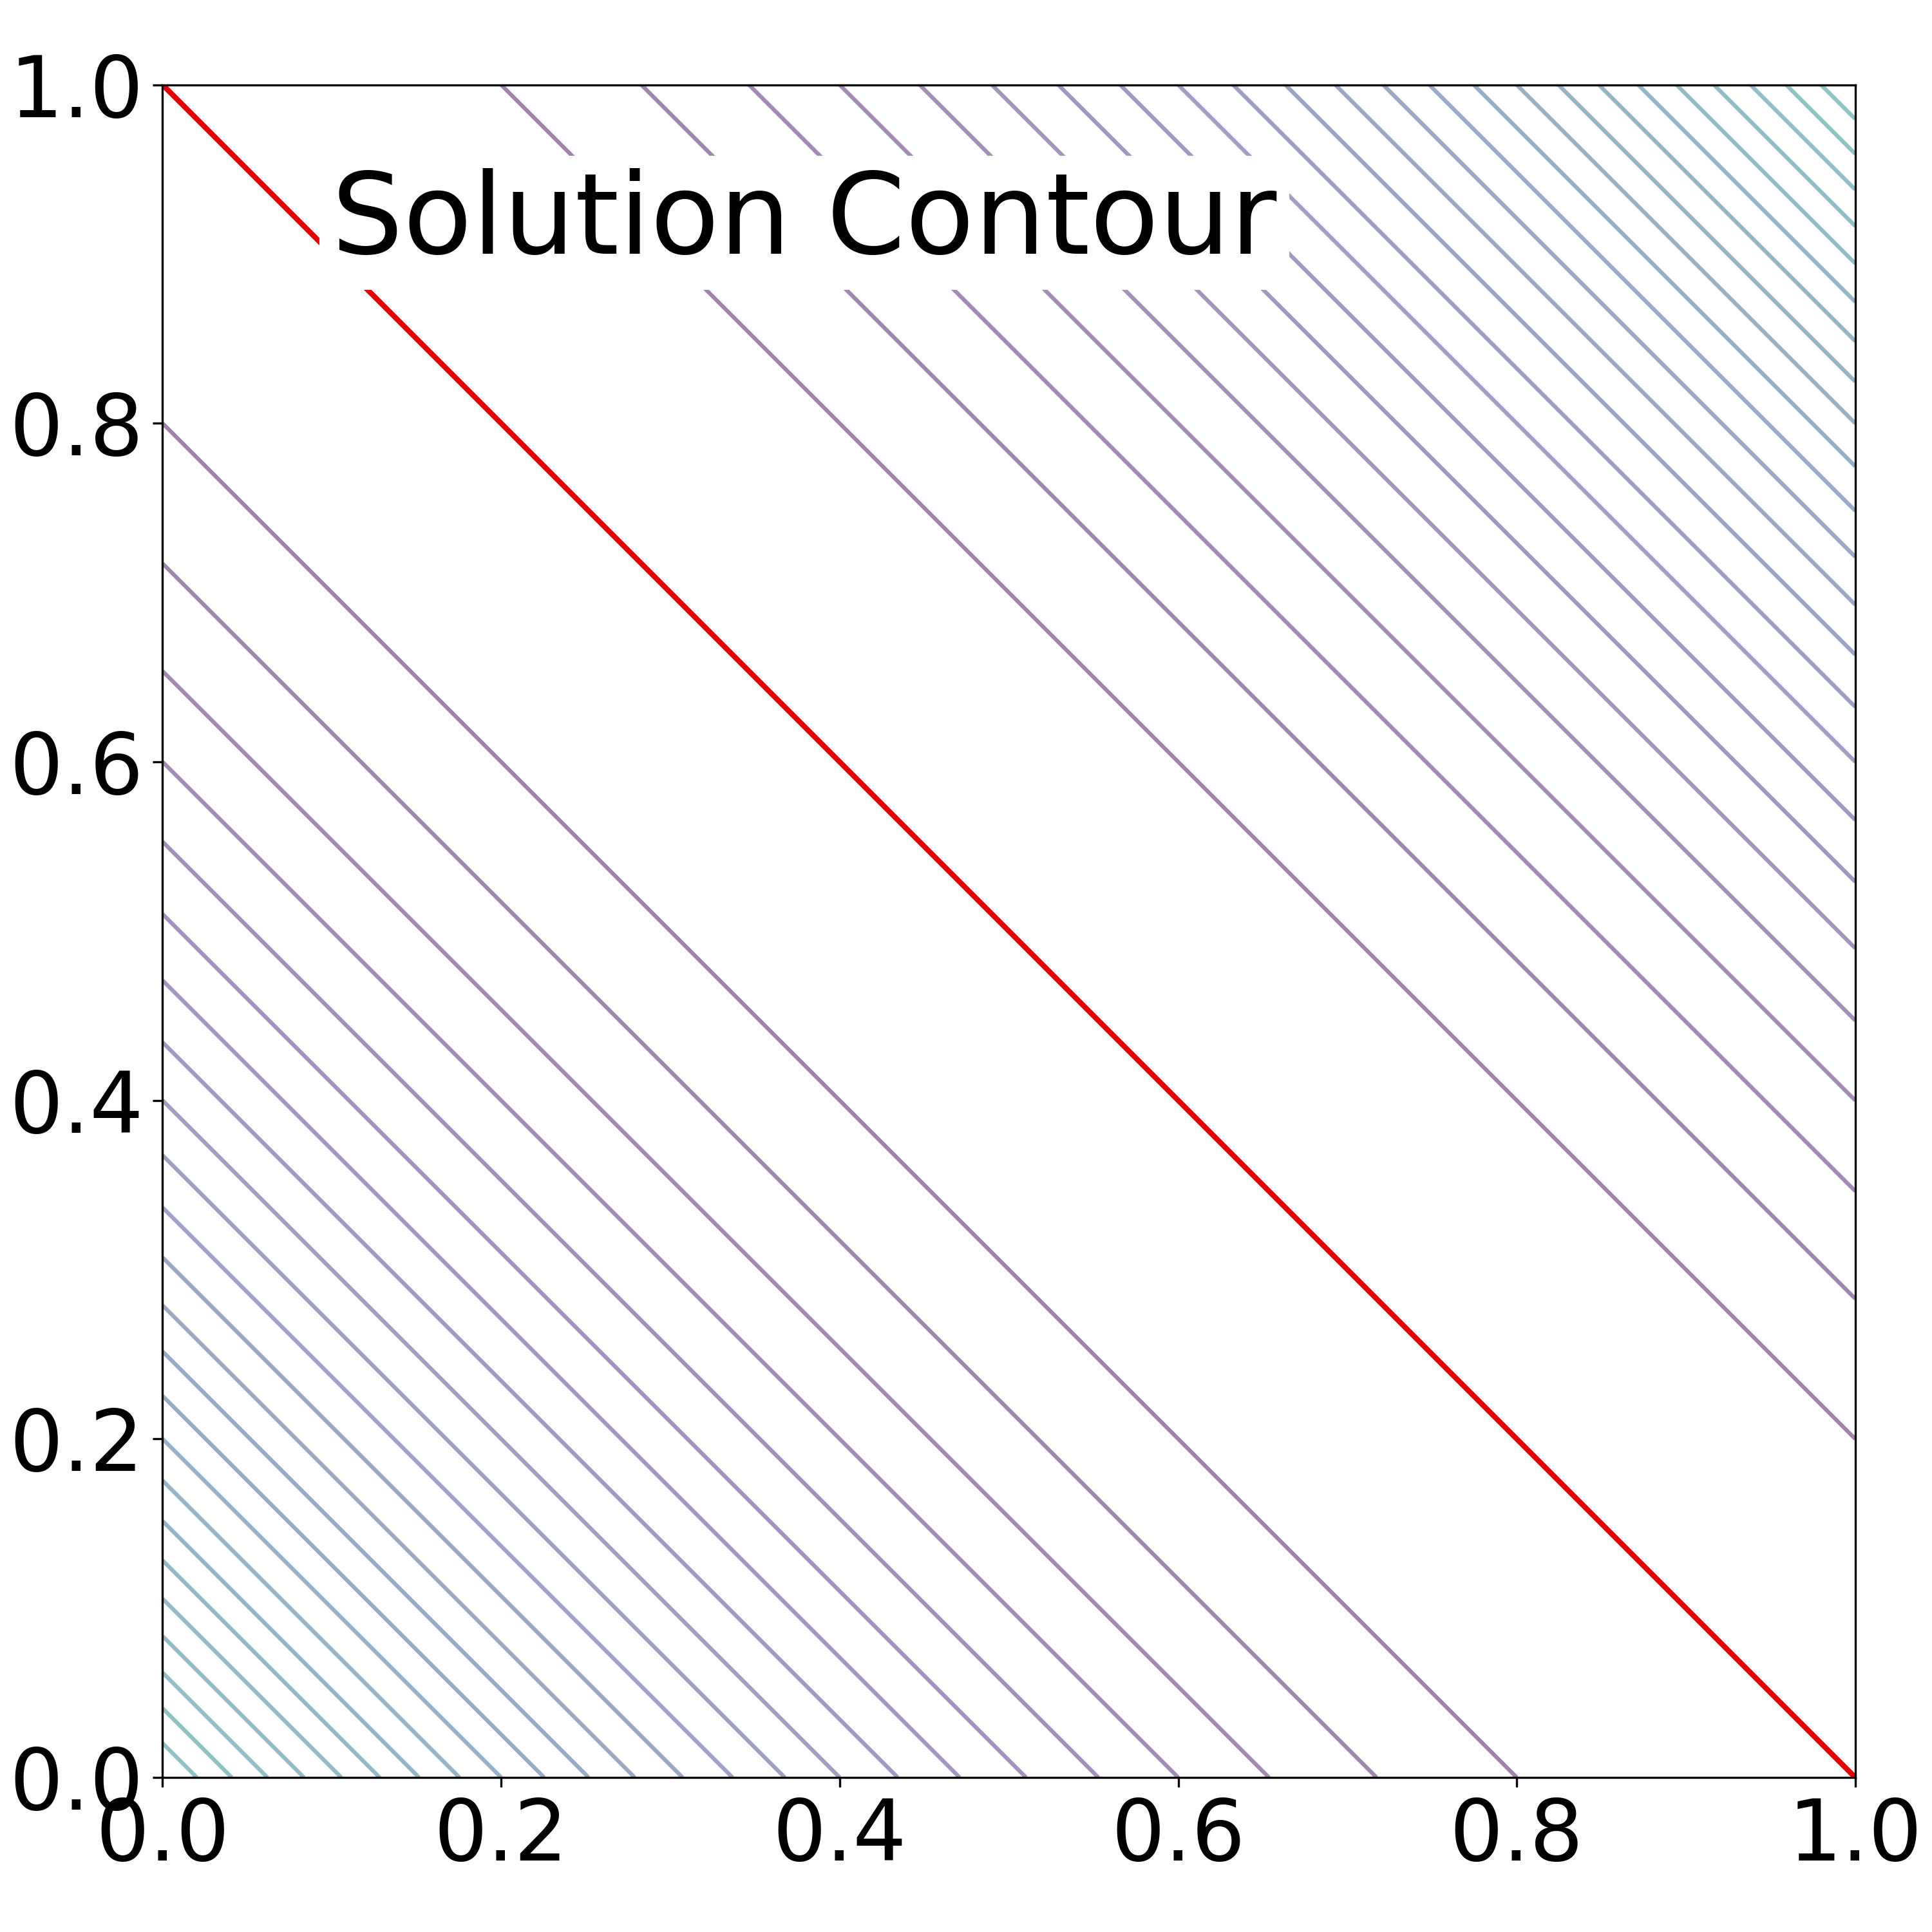
\includegraphics[width=0.25\linewidth]{figures/data_mismatch_contour.png}}
      {data mismatch}
    &
      \subf{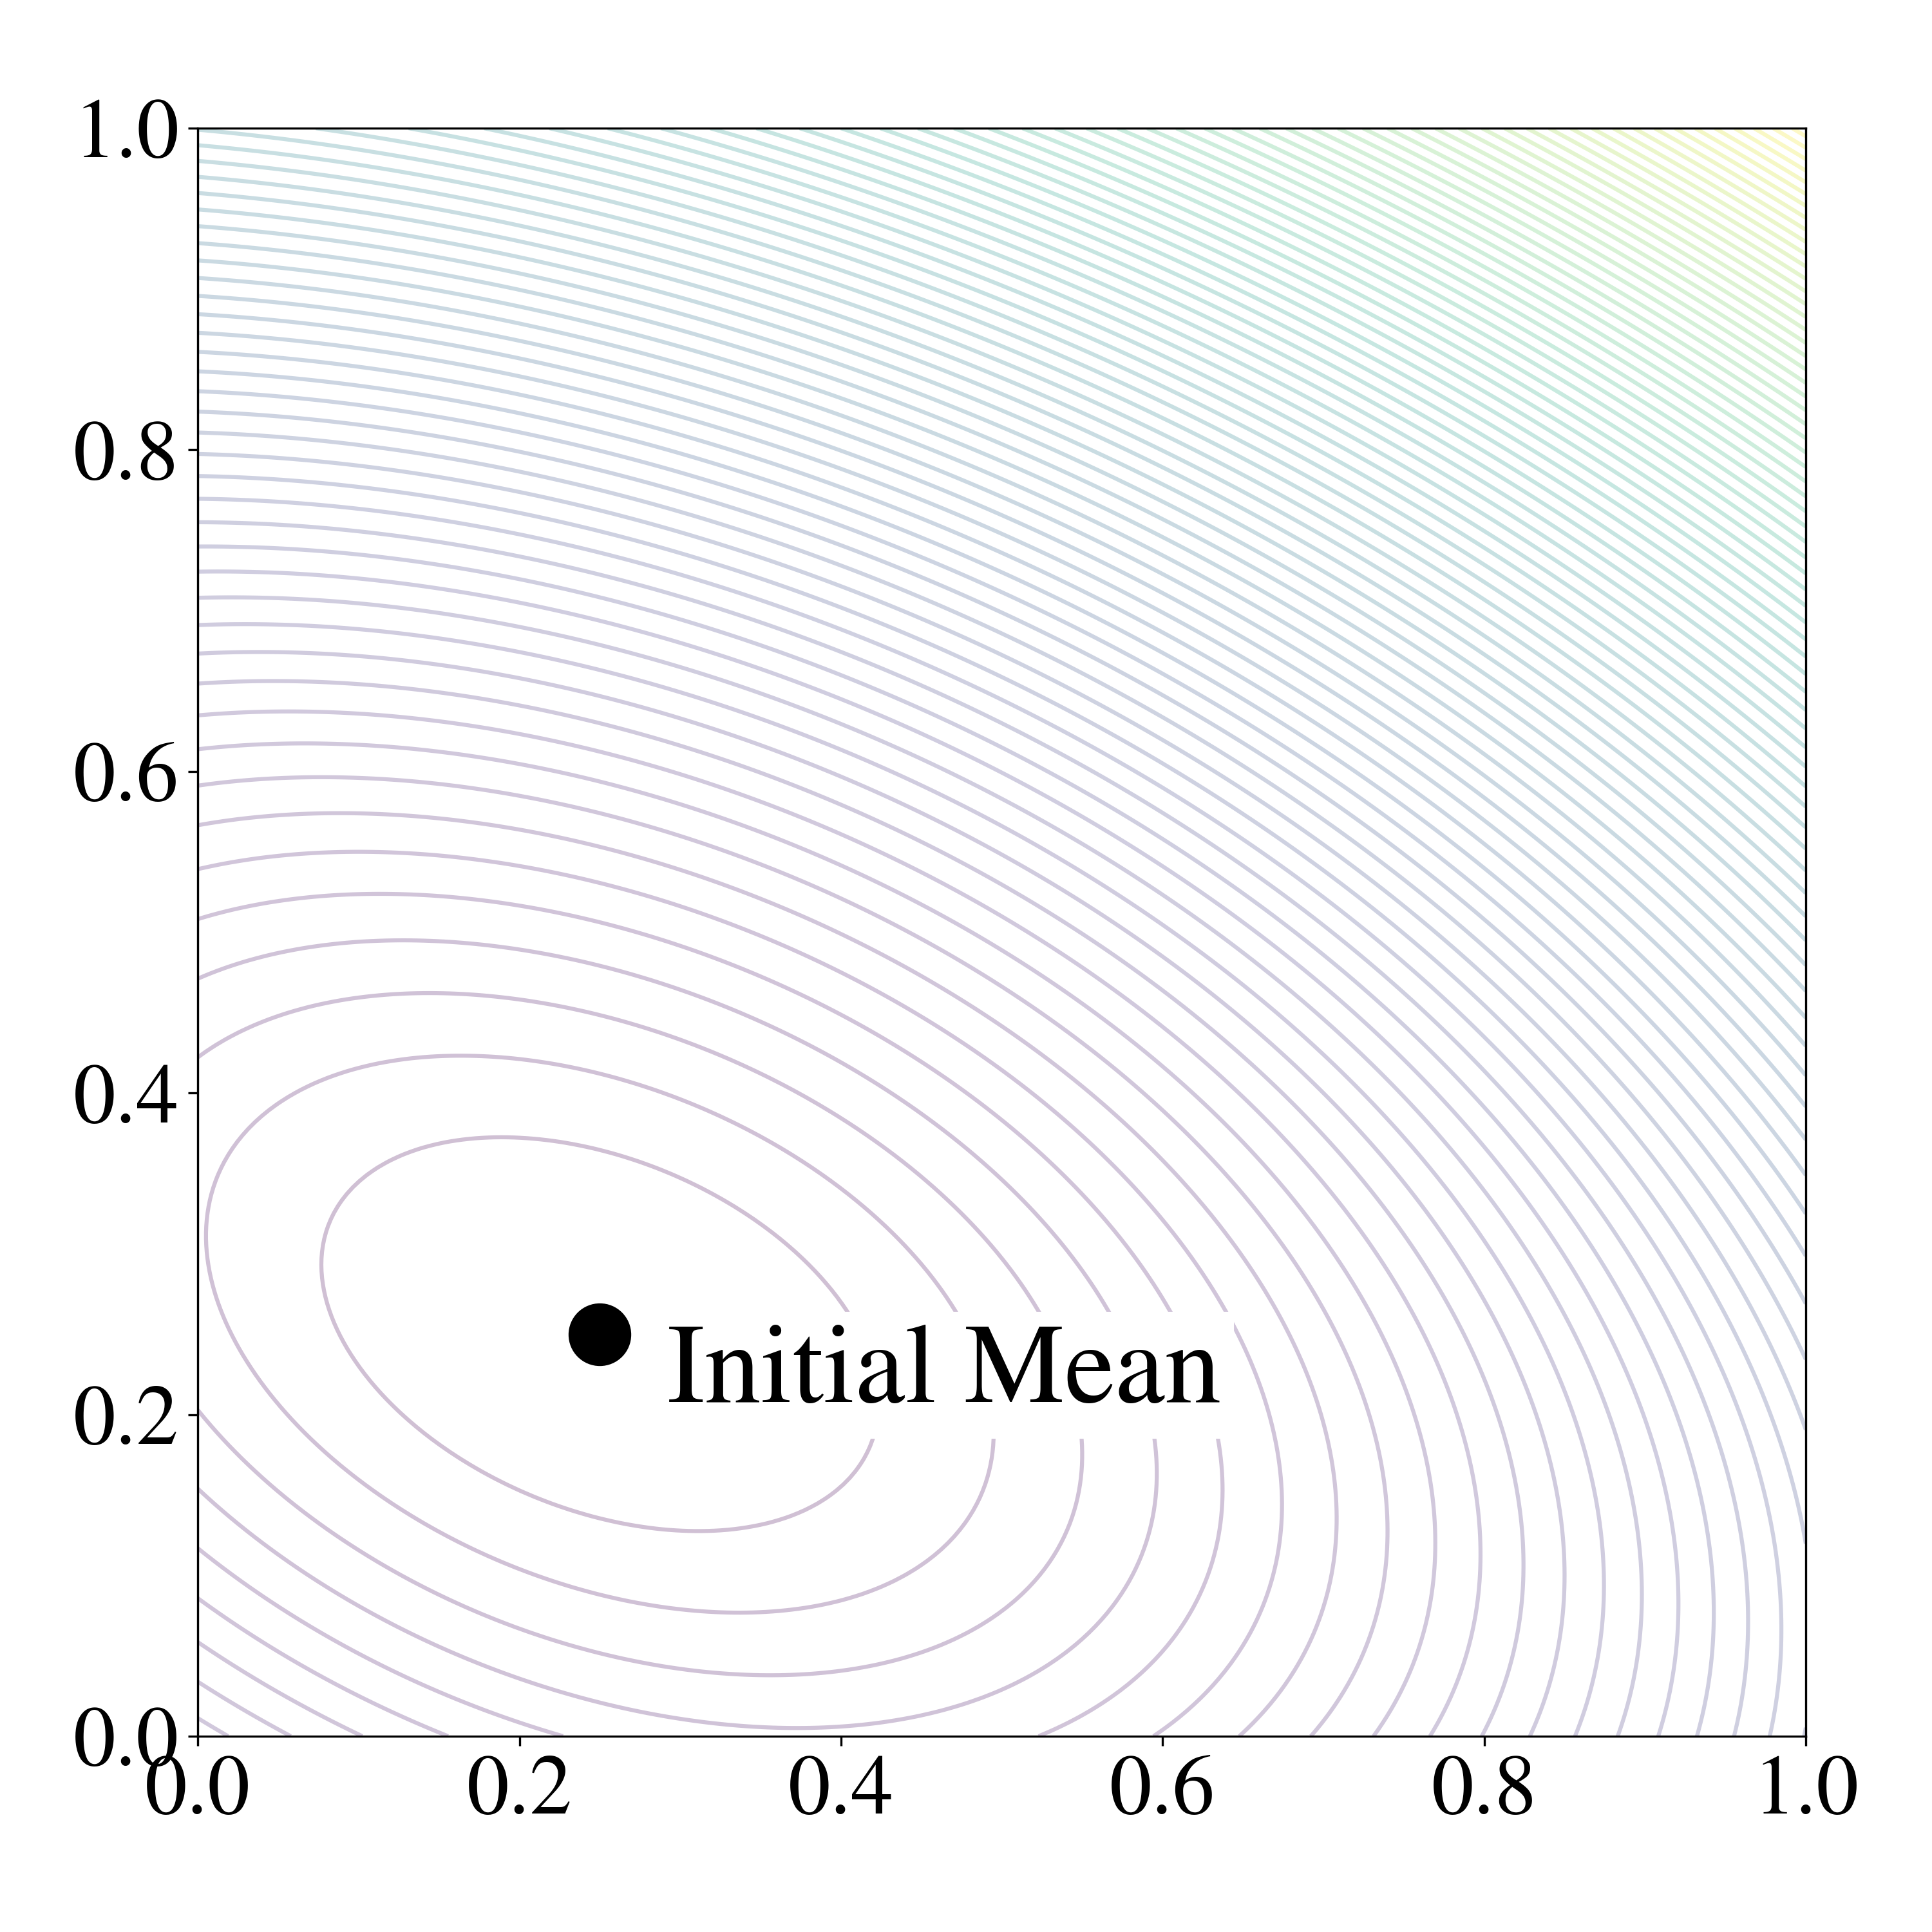
\includegraphics[width=0.25\linewidth]{figures/tikonov_contour.png}}
      {regularization}
    &
      \subf{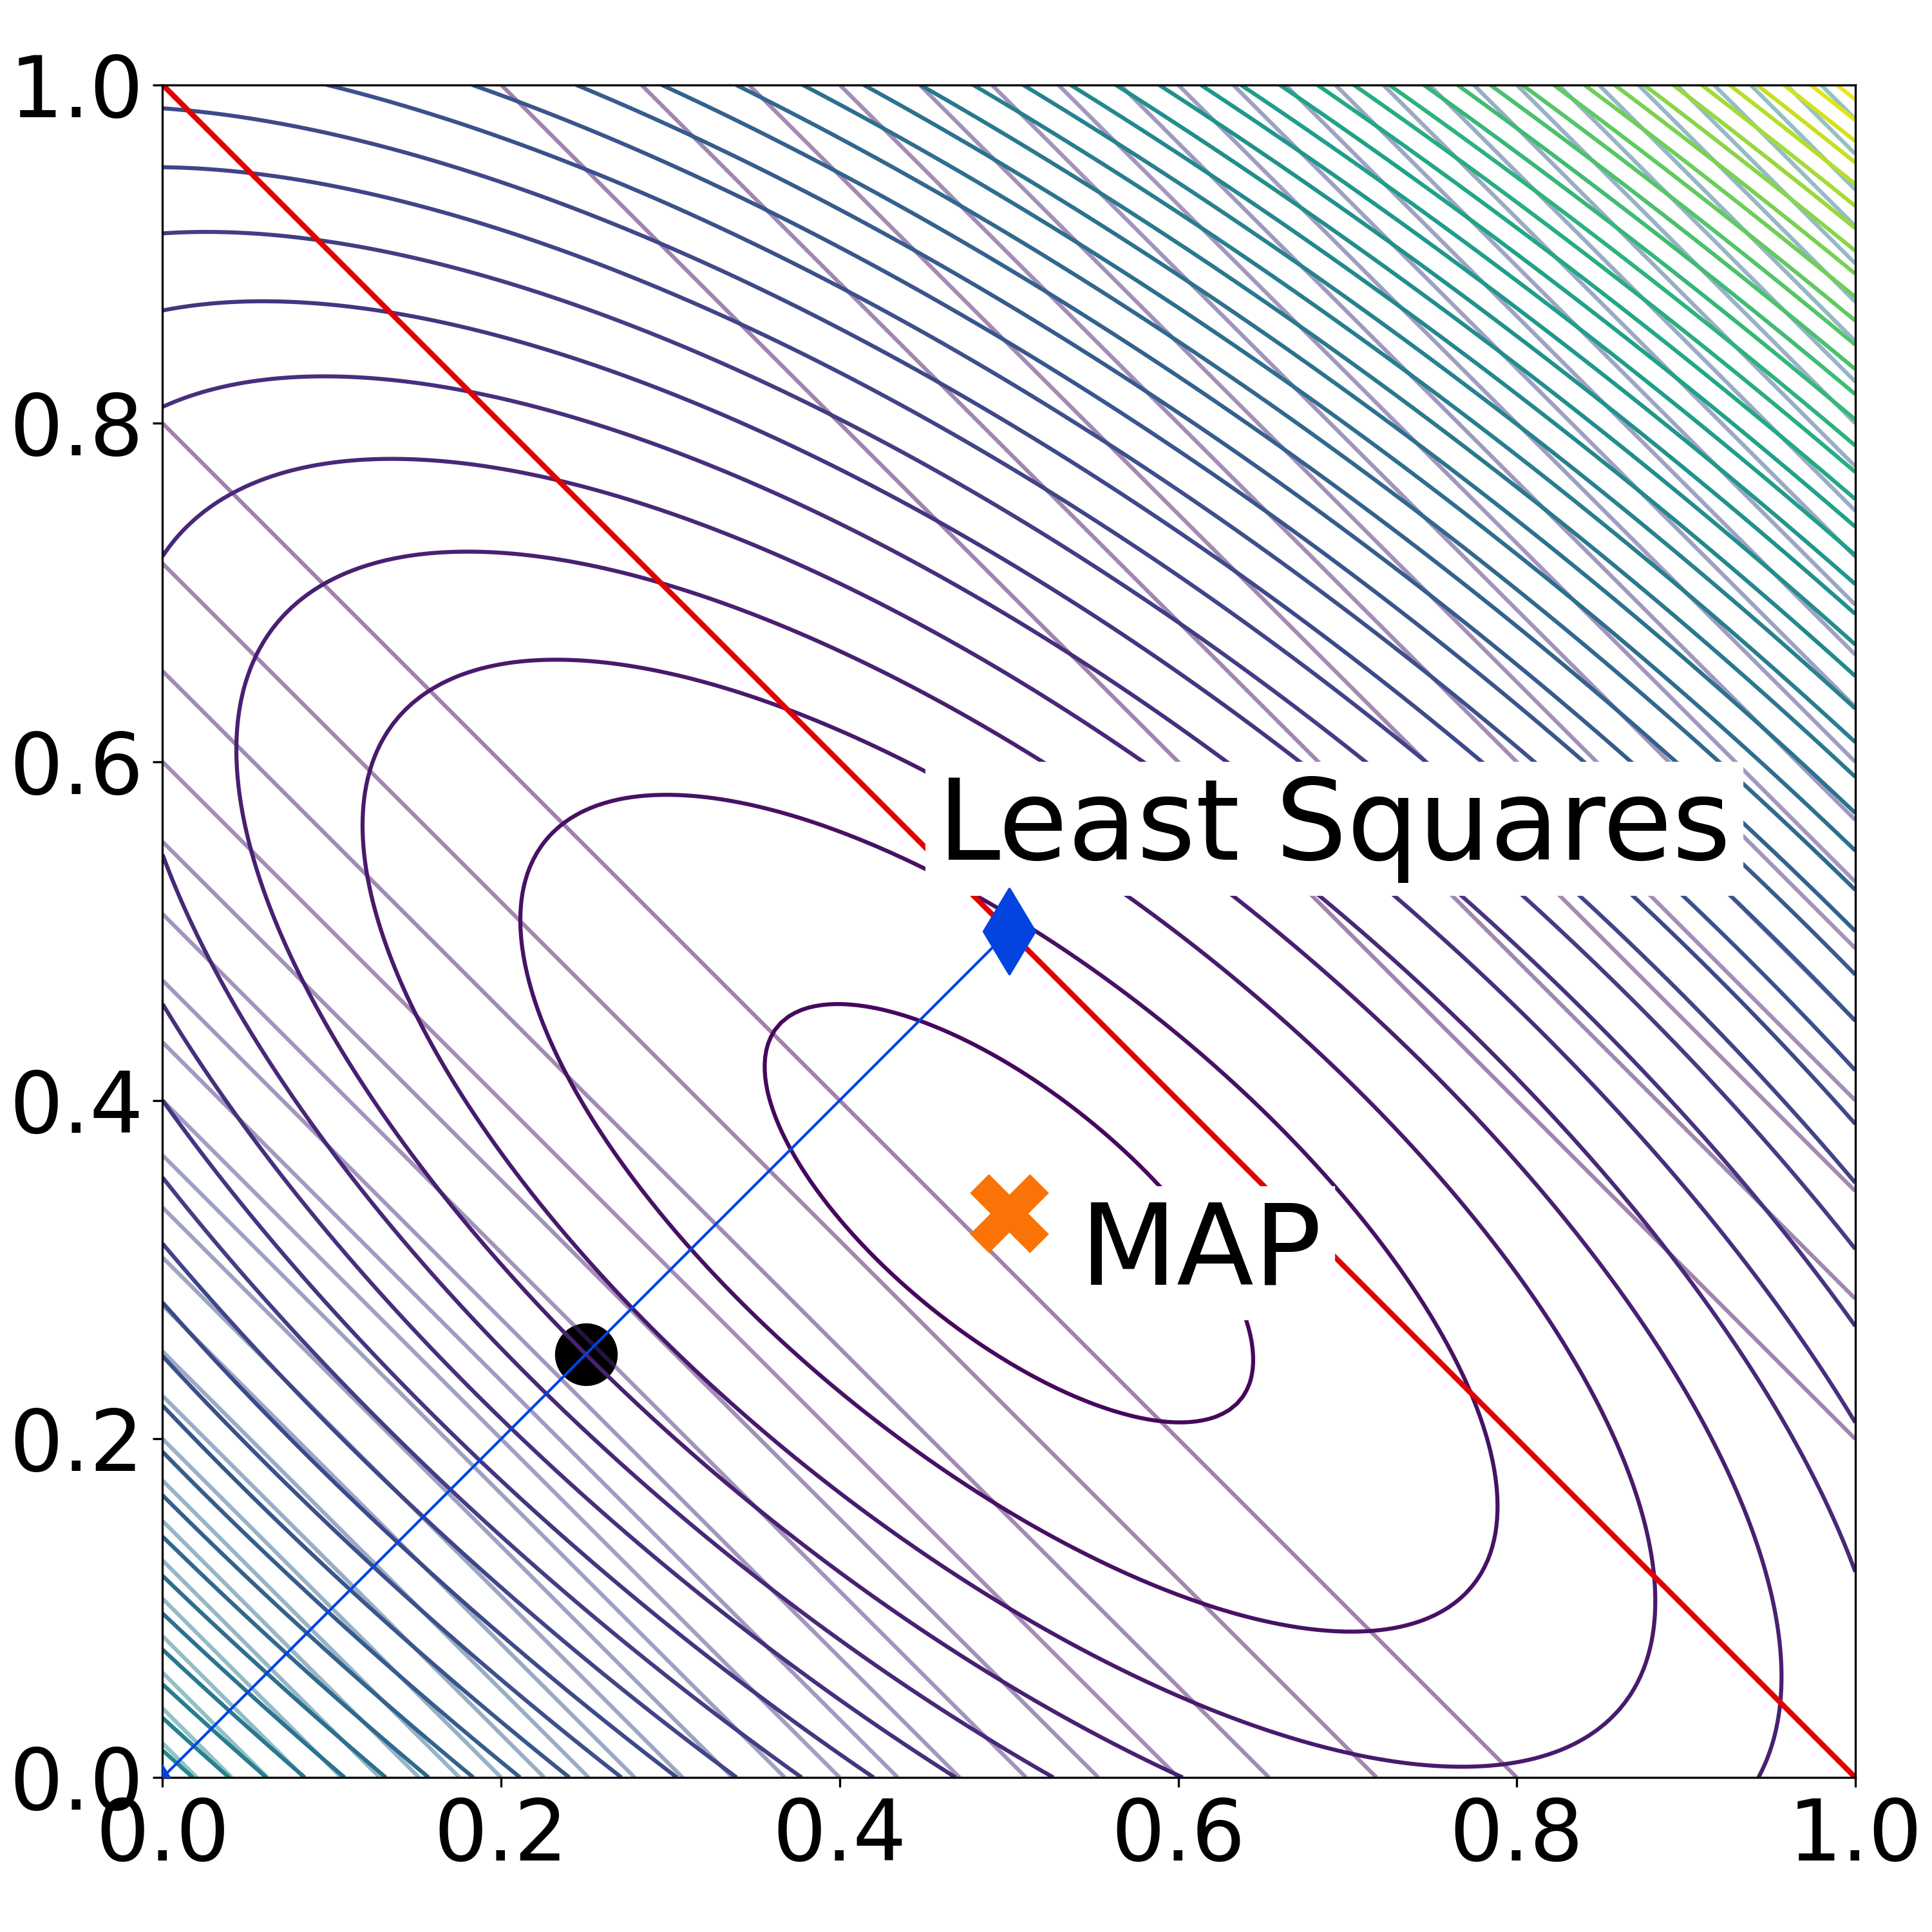
\includegraphics[width=0.25\linewidth]{figures/classical_solution.png}}
      {bayesian posterior}
    \\
    \hline
      \subf{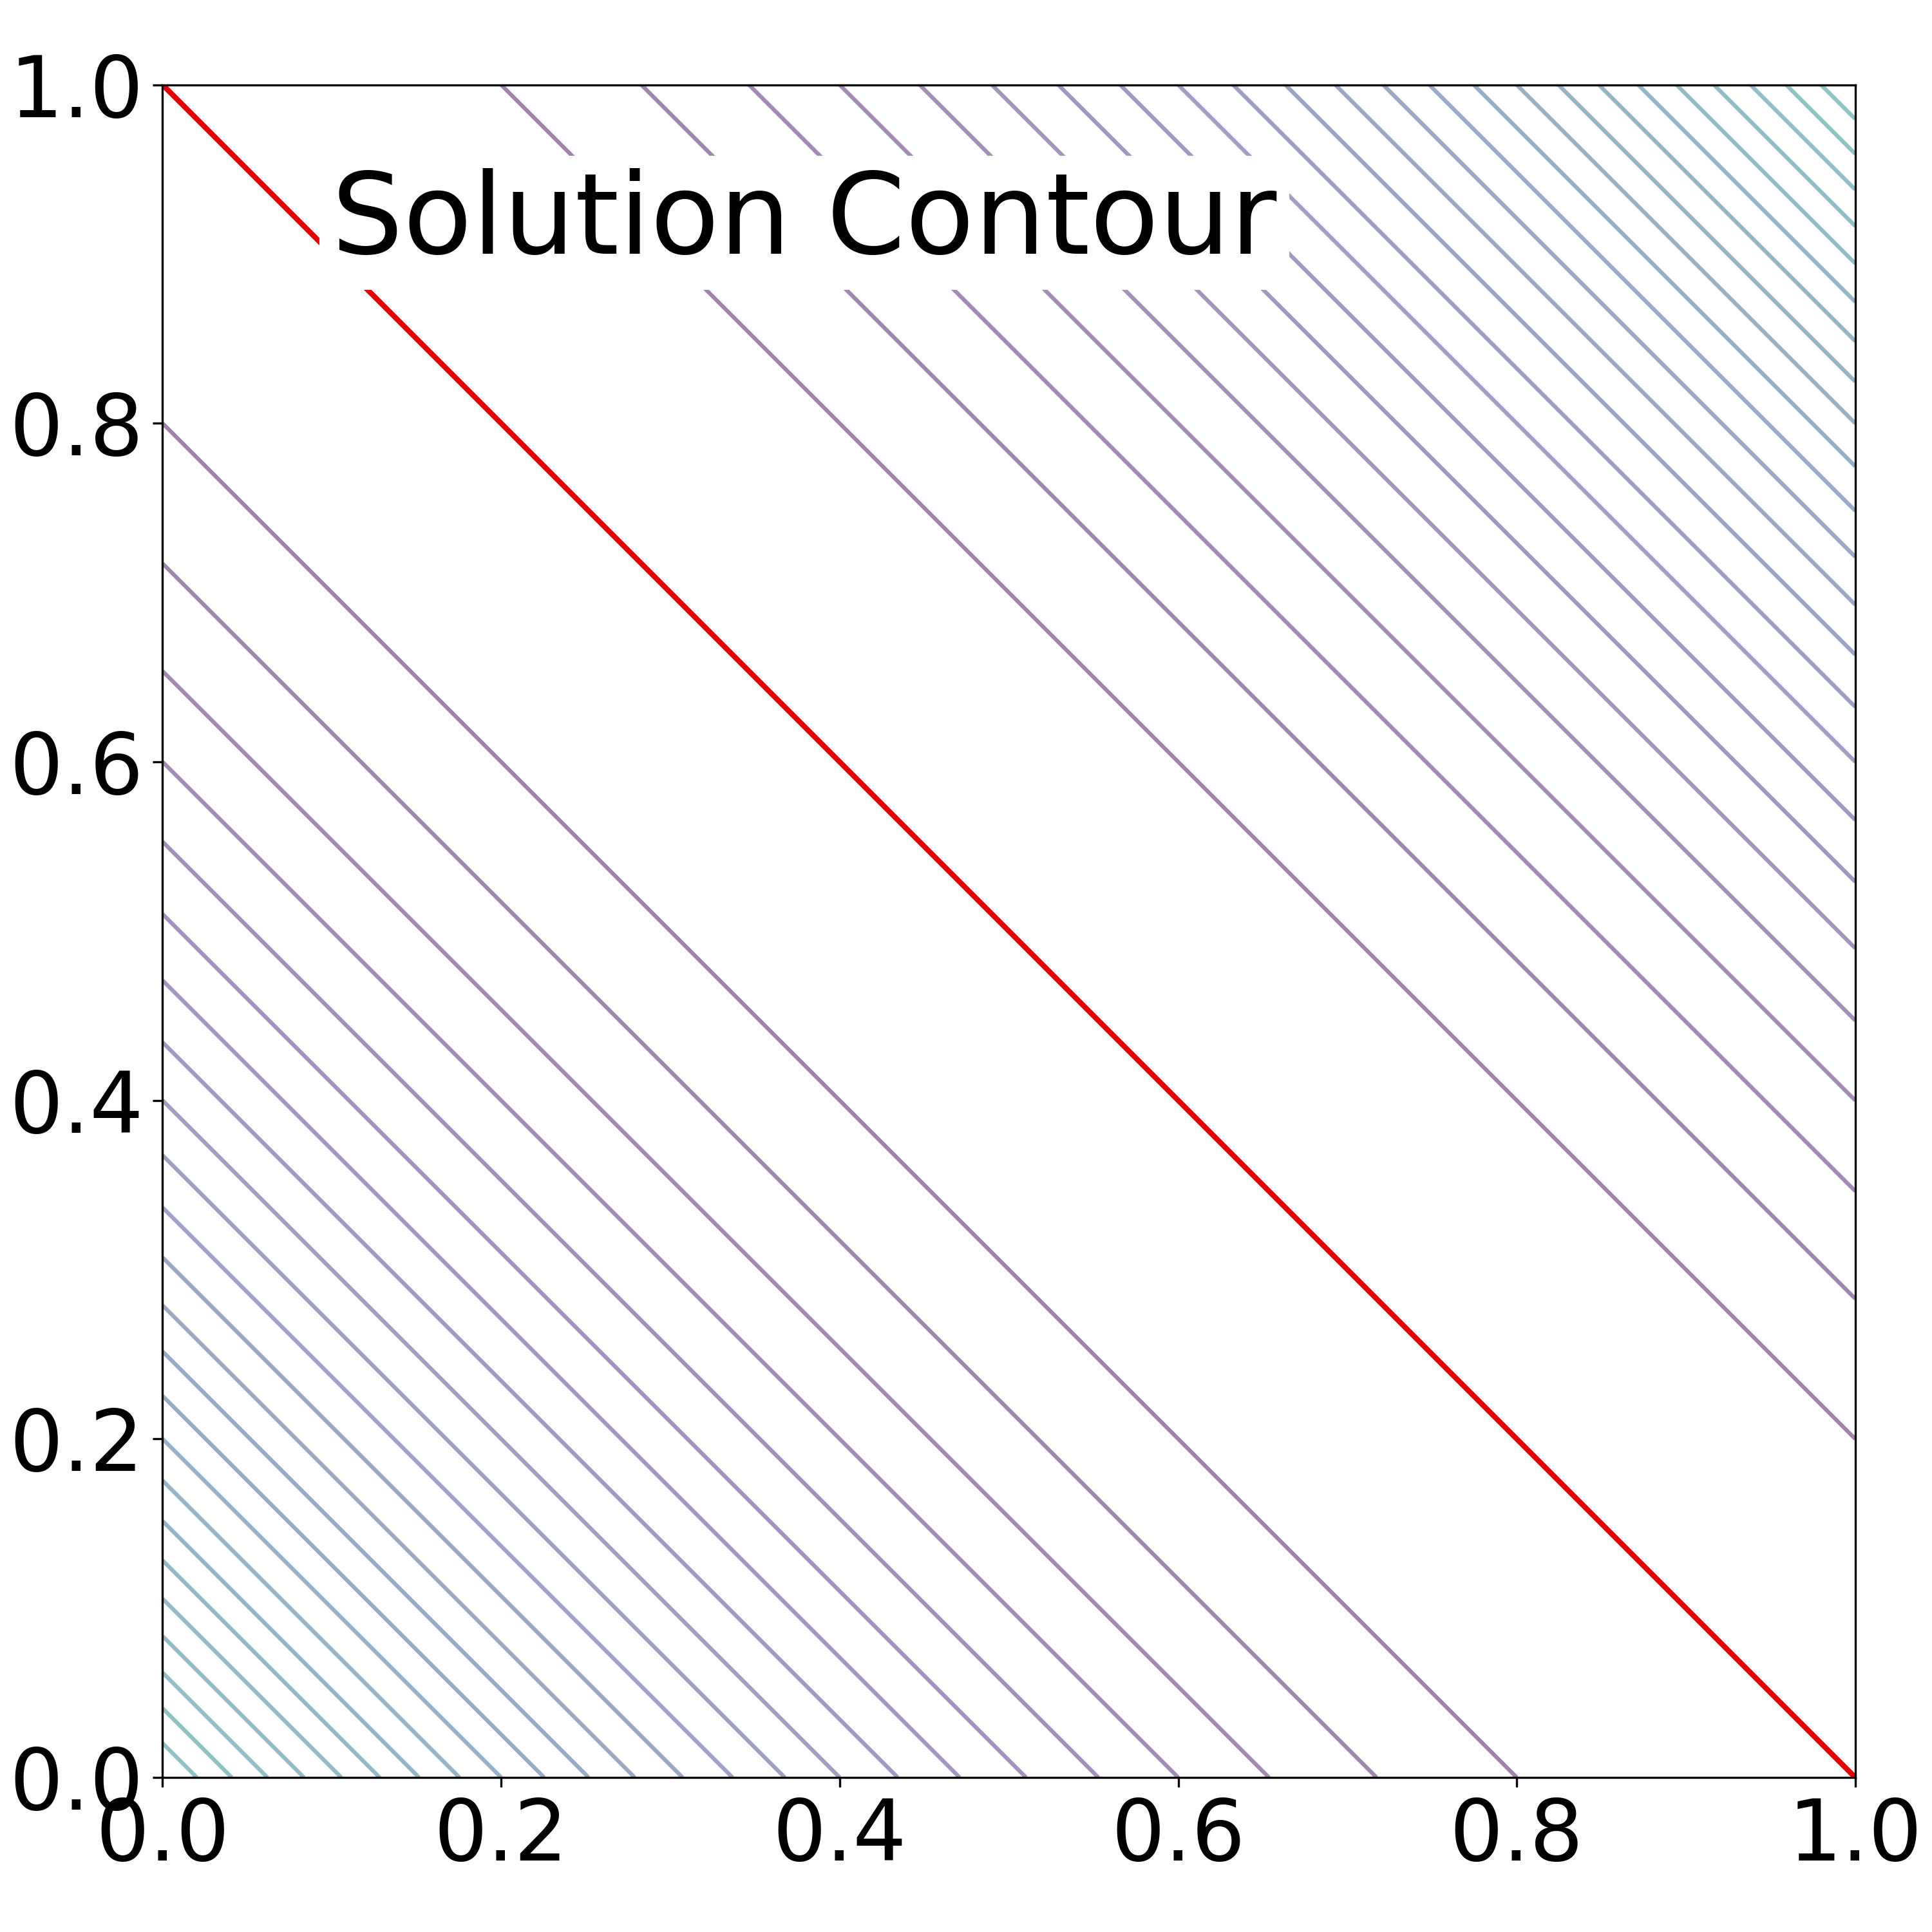
\includegraphics[width=0.25\linewidth]{figures/data_mismatch_contour.png}}
      {data mismatch}
    &
      \subf{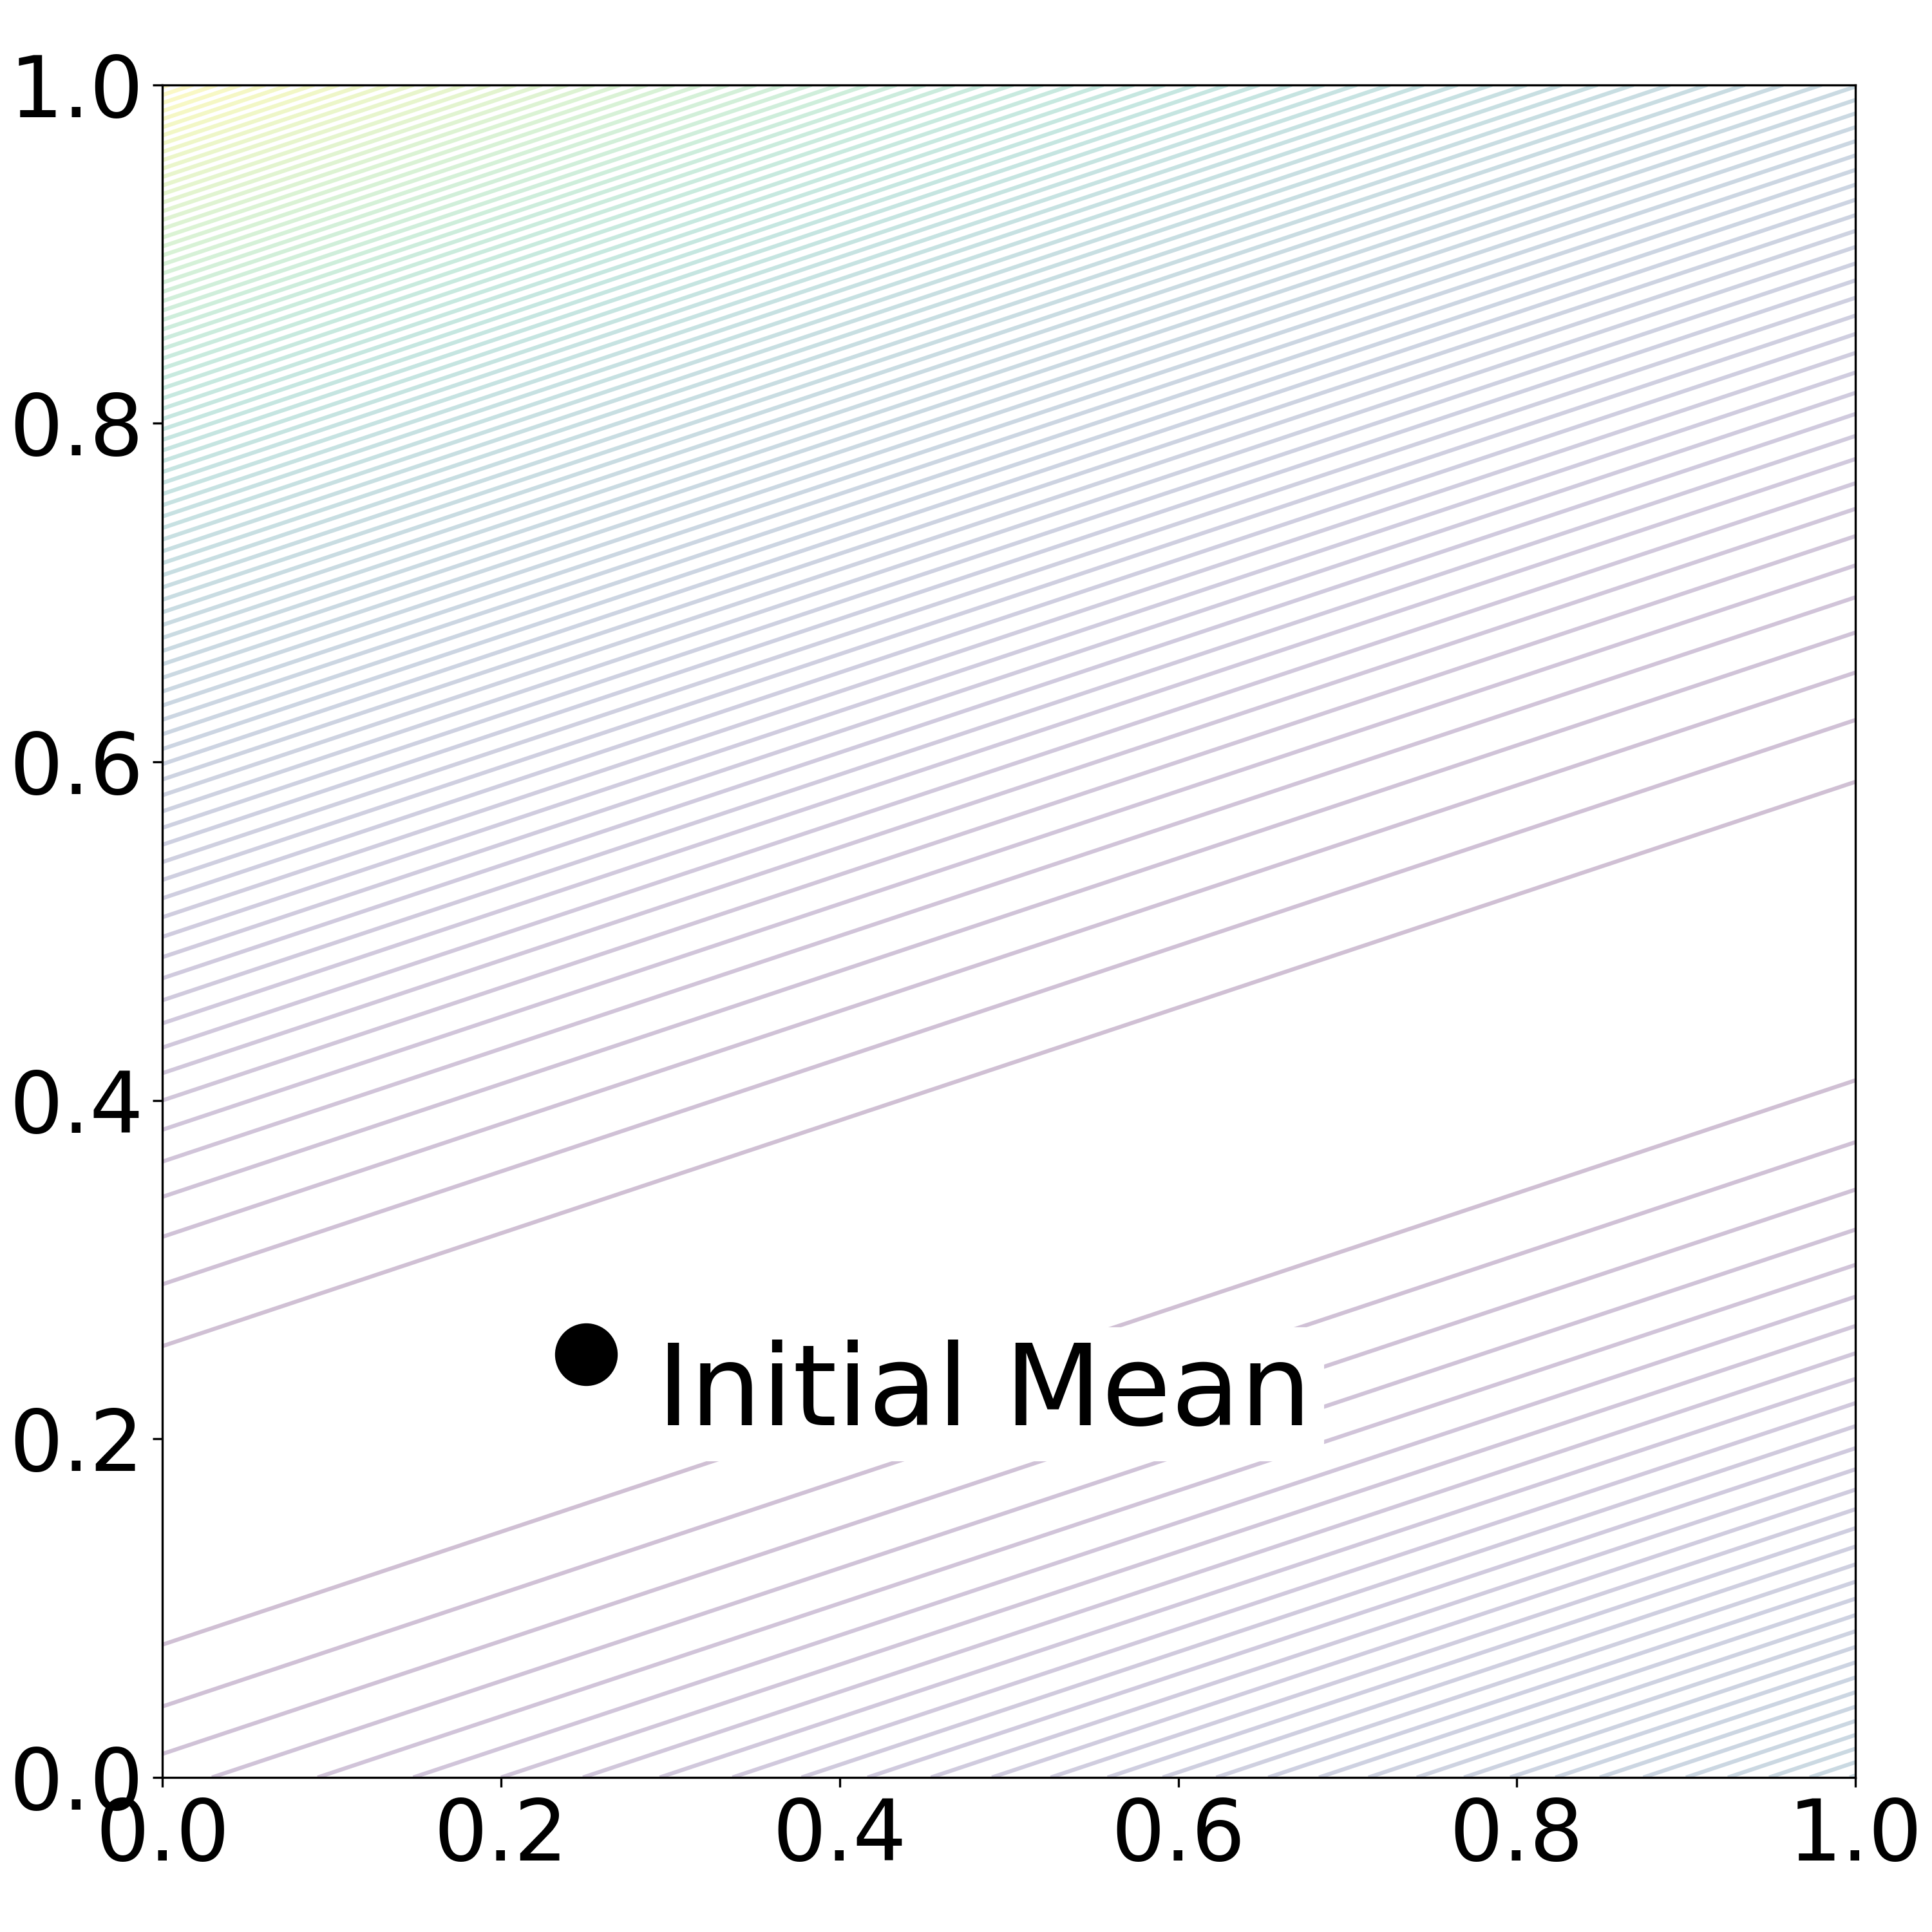
\includegraphics[width=0.25\linewidth]{figures/consistent_contour.png}}
      {modified regularization}
    &
      \subf{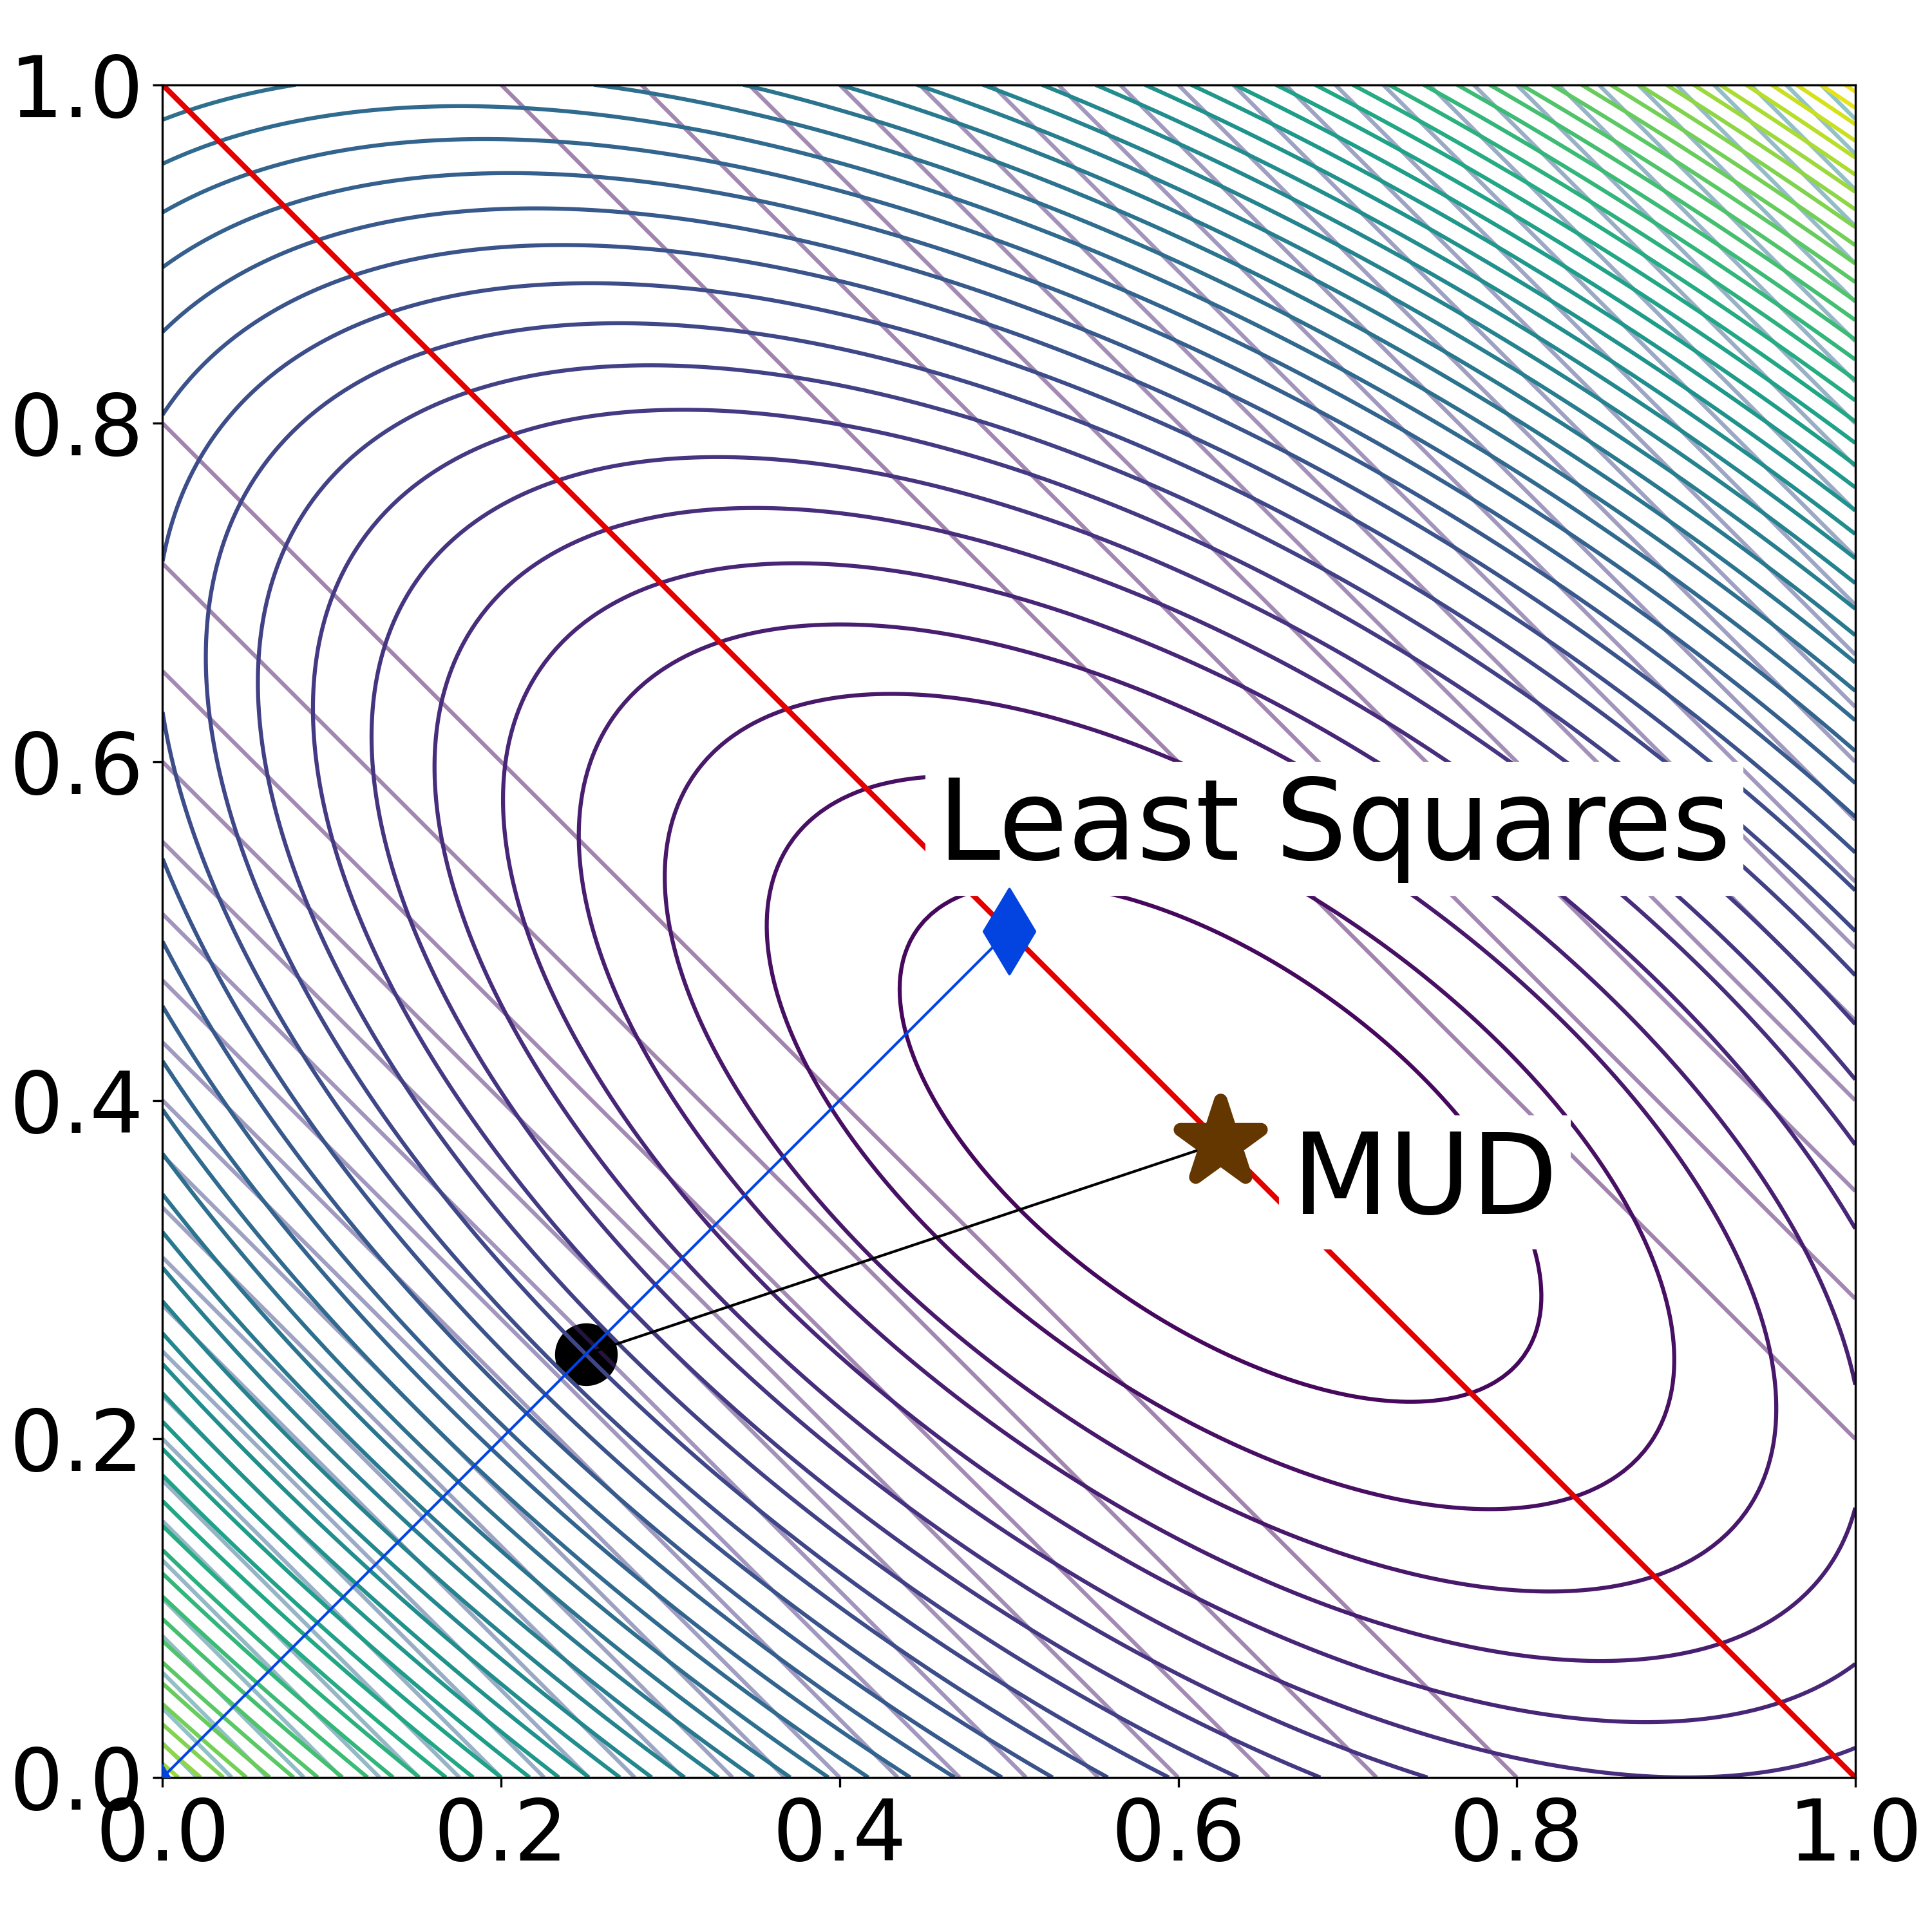
\includegraphics[width=0.25\linewidth]{figures/consistent_solution.png}}
       {updated density}
    \\
    \hline
  \end{tabular}
  %
  % \caption{Gaussian data mismatch for a 2-to-1 linear map (left plots). Gaussian initial/prior induce different regularization terms (middle plots), which leads to different optimization functions (right plots) and parameter estimates.}
  \label{fig:regularization}
\end{figure}


\end{figure}

\end{frame}


%%%%%%%%%%%%%%%%%%%%%%%%%%%%%%%%%%%%%%%%%%%%%%%%%%%%%%%%%%%
\subsection{Closed-Form Solutions}
%%%%%%%%%%%%%%%%%%%%%%%%%%%%%%%%%%%%%%%%%%%%%%%%%%%%%%%%%%%

\begin{frame}

\begin{itemize}
\item Posterior covariance:

\begin{equation}\label{eq:map_cov}
  \Sigma_\text{post} := ( A^\top {\Sigma}_\text{obs}^{-1} A + \initialCov^{-1} )^{-1}
\end{equation}

\bigskip
\item Using Woodbury identity and~\eqref{eq:predictCov}:

\begin{equation}\label{eq:map_cov_analytical}
  \Sigma_\text{post} = \initialCov - \initialCov A^\top \left[\predictedCov + \observedCov\right]^{-1} A \initialCov
\end{equation}

\bigskip
\item Interpretation: $\Sigma_\text{post}$ is a rank $d$ correction (or update) of $\initialCov$.

\bigskip
\item $\predictedCov + \observedCov$ is invertible because it is the sum of two s.p.d matrices. \\

\bigskip
\item Rewrite using analytical expression for the MAP point:

\begin{equation}\label{eq:map-point-analytical}
  \param^{\text{MAP}} = \param_0 + \Sigma_\text{post} A^\top \observedCov^{-1} (\observedMean - b - A\param_0).
\end{equation}

\end{itemize}

\end{frame}


%%%%%%%%%%%%%%%%%%%%%%%%%%%%%%%%%%%%%%%%%%%%%%%%%%%%%%%%%%%
\begin{frame}[t]{\it The one where we make some convenient manipulations.}
\begin{itemize}
  \item Let

  \begin{equation}\label{eq:eff_reg}
  	R := \nolinebreak \initialCov^{-1} - \nolinebreak A^\top \predictedCov^{-1} A.
  \end{equation}

  \bigskip
  \item Using this $R$, rewrite $J(\param)$ as

  \begin{equation}\label{eq:dci-objective-alt}
  J(\param):= \norm{\observedMean - Q(\param)}_{\observedCov^{-1}}^2 + \norm{\param - \param_0}_{R}^2.
  \end{equation}

  \bigskip
  \item $R$ is the {\em effective regularization} in $J(\param)$ in the DCI framework:

  \begin{equation}
  	\updatedCov := \left(A^\top \observedCov^{-1} A + R\right)^{-1}
  \end{equation}

  \bigskip
  \item Since $R$ is not invertible, Woodbury's identity cannot be applied (yet).

\end{itemize}

\end{frame}

%%%%%%%%%%%%%%%%%%%%%%%%%%%%%%%%%%%%%%%%%%%%%%%%%%%%%%%%%%%
\begin{frame}[t]{\it The one where we make some convenient manipulations.}
\begin{itemize}
  \item \emph{Using linear algebra ...}

  \begin{equation}\label{eq:updatedCov_final}
  	\updatedCov = \initialCov - \initialCov A^\top \predictedCov^{-1}\left[\predictedCov-\observedCov\right]\predictedCov^{-1}A\initialCov.
  \end{equation}

  \bigskip
  \bigskip
  \item Substitute $\updatedCov$ for $\Sigma_\text{post}$ in \eqref{eq:map-point-analytical}:

  \begin{equation}\label{eq:mud-point-analytical-alt}
  \param^{\text{MUD}} = \param_0 + \updatedCov A^\top \observedCov^{-1} (\observedMean - b - A\param_0).
  \end{equation}

  \bigskip
  \bigskip
  \item Substituting~\eqref{eq:updatedCov_final} into~\eqref{eq:mud-point-analytical-alt} and simplifying, we have

  \begin{equation}\label{eq:mud-point-analytical-final}
  	\mudpt = \param_0 + \initialCov A^\top \predictedCov^{-1}(\observedMean - b - A\param_0).
  \end{equation}

\end{itemize}

\end{frame}

%%%%%%%%%%%%%%%%%%%%%%%%%%%%%%%%%%%%%%%%%%%%%%%%%%%%%%%%%%%
\begin{frame}

\begin{thm}\label{thm:MUD_existence_uniqueness}

Suppose  $Q(\param)=A\param+b$ for some full rank $A\in\RR^{d\times p}$ with $d\leq p$ and $b\in\RR^d$.

If $\initial \sim N(\param_0,\initialCov)$, $\observed\sim N(\observedMean,\observedCov)$, and the predictability assumption holds, then

\begin{enumerate}[(a)]
  \item There exists a unique $\mudpt$.
  \item $Q(\mudpt) = \observedMean$.
  \item If $d=p$, $\mudpt$ is given by $A^{-1}$. If $d<p$, $\mudpt$ is given by~\eqref{eq:mud-point-analytical-final} and the covariance associated with this point is given by~\eqref{eq:updatedCov_final}.
\end{enumerate}
\end{thm}

\end{frame}

%%%%%%%%%%%%%%%%%%%%%%%%%%%%%%%%%%%%%%%%%%%%%%%%%%%%%%%%%%%
\begin{frame}{\it The one where we address a key assumption}

\begin{itemize}
  \item Predictability Assumption: $\predicted$ is a dominating measure for $\observed$
  \bigskip
  \bigskip
  \item Linear case: involves eigenvalues of covariances:
  \bigskip
    \begin{itemize}
      \item min eigenvalue $\predictedCov$ > max eigenvalue $\observedCov$
    \end{itemize}
\end{itemize}
\end{frame}

%%%%%%%%%%%%%%%%%%%%%%%%%%%%%%%%%%%%%%%%%%%%%%%%%%%%%%%%%%%
\subsection{Impact of Information Content}
%%%%%%%%%%%%%%%%%%%%%%%%%%%%%%%%%%%%%%%%%%%%%%%%%%%%%%%%%%%

\begin{frame}{\it The one where we show how rank and dimension impact our solutions.}
\centering

\begin{figure}[htbp]
\hbox{
  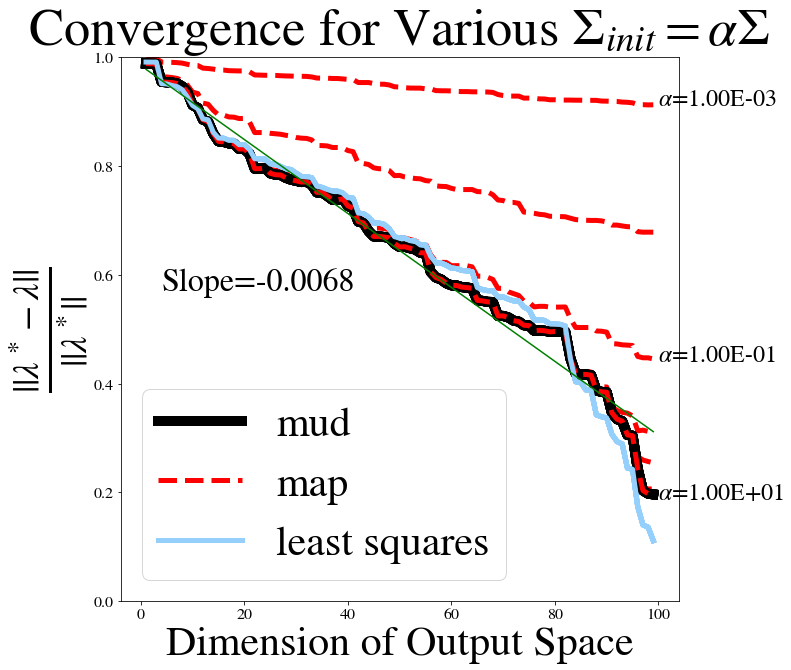
\includegraphics[width=0.5\linewidth]{figures/lin/lin-dim-cov-convergence}
  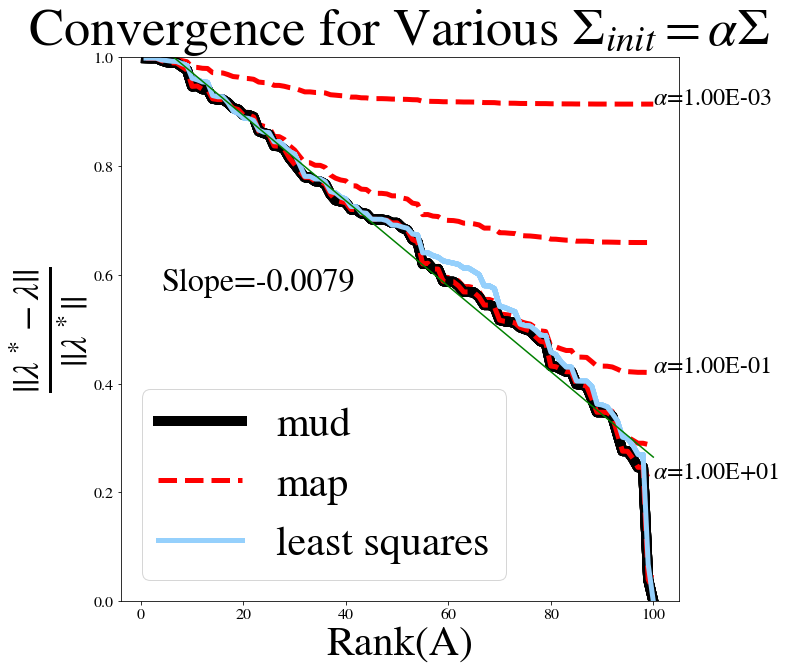
\includegraphics[width=0.5\linewidth]{figures/lin/lin-rank-cov-convergence}
}
% \caption{
% 	Relative errors between $\paramref$ and (i) the least squares solution obtained through {\tt numpy}'s {\tt linalg.pinv} module, (ii) the closed-form solution for the MUD point given in Eq~\eqref{eq:mud-point-analytical-final}, and (iii) the MAP point.
%   (Left): Error for increasing dimensions of $D$ for $A$ taken to be a Gaussian Random Map.
%   (Right): Error for increasing row-rank of $A$, generated with Gaussian vectors and a SVD.
% }
\label{fig:lin-error}
\end{figure}

Example: scaling random diagonal initial covariances

\end{frame}


%%%%%%%%%%%%%%%%%%%%%%%%%%%%%%%%%%%%%%%%%%%%%%%%%%%%%%%%%%%
\subsection{Data-Driven QoI Maps}
%%%%%%%%%%%%%%%%%%%%%%%%%%%%%%%%%%%%%%%%%%%%%%%%%%%%%%%%%%%

\begin{frame}{\it The one where we leverage this framework for general streams of data.}

\begin{itemize}
  \item Measurement devices $M_j$ generating repeated noisy data, $1\leq j\leq d$.

  \bigskip
  \item $d_{j,i}$ is the $i$th noisy datum for the $j$th measurement, where $1\leq i\leq N_j$.

  \bigskip
  \item Unbiased additive error model for the measurement noise:

  \begin{equation}\label{eq:obs_data_error}
  	d_{j,i} = M_j(\paramref) + \xi_i, \ \xi_i\sim N(0,\sigma_j^2), \ \ 1\leq i\leq N_j.
  \end{equation}

\end{itemize}

\bigskip
\bigskip
\centering
{\it We now construct a $d$-dimensional vector-valued map from data obtained on the $d$ measurement devices.}

\end{frame}


%%%%%%%%%%%%%%%%%%%%%%%%%%%%%%%%%%%%%%%%%%%%%%%%%%%%%%%%%%%
\begin{frame}{\it The one with the Weighted Mean Error (WME) map $Q_\text{WME}(\param)$.}

\begin{equation}\label{eq:qoi_WME}
	Q_{\text{WME},j}(\param) := \frac{1}{\sqrt{N_j}} \sum_{i=1}^{N_j} \frac{M_j(\param)-d_{j,i}}{\sigma_j}.
\end{equation}

\bigskip
\begin{itemize}
  \item $Q_{\text{WME},j}(\paramref)$ is the sample avg of $N_j$ draws from an i.i.d.~$N(0,N_j)$.

  \bigskip
  \item Observed data are generated according to fixed (truth) $\paramref$ in \eqref{eq:obs_data_error}.

  \bigskip
  \item For each component, $Q_{\text{WME},j}(\paramref) \sim N(0, 1)$.

  \bigskip
  \item $\observed$ is a $N(\mathbf{0}_{d\times 1},\mathbf{I}_{d\times d})$ due to the structure of $Q_\text{WME}(\param)$.

\end{itemize}


\end{frame}

%%%%%%%%%%%%%%%%%%%%%%%%%%%%%%%%%%%%%%%%%%%%%%%%%%%%%%%%%%%
\begin{frame}{\it The one where measurements impact the predictability assumption.}

\begin{itemize}

	\item The $j$th diagonal component of $\predictedCov$ is given by the predicted variance associated with using the scalar-valued $Q_{\text{WME},j}$.

	\bigskip
  \item The associated predicted variance for the $j$th component is given by:

	\bigskip
  \begin{equation}
  	\frac{N_j}{\sigma_j^2} M_j\initialCov M_j^\top.
  \end{equation}

  \bigskip
  \item $\initialCov$ non-degenerative and $M_j$ non-trivial row vector, which implies that the {\it \bf predicted variance grows linearly} with $N_j$.\\

\end{itemize}

\bigskip
\bigskip
\centering
{\it The following result is now an immediate consequence of Theorem~\ref{thm:MUD_existence_uniqueness}.}
\end{frame}

%%%%%%%%%%%%%%%%%%%%%%%%%%%%%%%%%%%%%%%%%%%%%%%%%%%%%%%%%%%
\begin{frame}

\begin{corollary}\label{cor:MUD_wme}
If $\initial \sim N(\param_0,\initialCov)$ and data are obtained for $d$ linearly independent measurements on $\pspace$ with an additive noise model with i.i.d. Gaussian noise for each measurement, then {\bf there exists a minimum number of data points obtained for each of the measurements} such that there exists a unique $\mudpt$ and $Q_\text{WME}(\mudpt) = 0$.
\end{corollary}

\end{frame}



%%%%%%%%%%%%%%%%%%%%%%%%%%%%%%%%%%%%%%%%%%%%%%%%%%%%%%%%%%%
\subsection{Nonlinear Examples}
%%%%%%%%%%%%%%%%%%%%%%%%%%%%%%%%%%%%%%%%%%%%%%%%%%%%%%%%%%%

%%%%%%%%%%%%%%%%%%%%%%%%%%%%%%%%%%%%%%%%%%%%%%%%%%%%%%%%%%%
\begin{frame}{\it The one where we violate some assumptions (and see what happens).}
%\vskip 25pt

Consider the exponential decay problem with uncertain decay rate $\param$:

\bigskip
$$
\begin{cases}
\frac{\partial u}{\partial t} & = \param u(t), \ 0<t\leq 3, \\ u(0) &= 0.75,
\end{cases}
$$

\bigskip
\bigskip
with solution

\begin{equation}
u(t;\param) = u_0\exp(-\param t), \; u_0 = 0.75 ,
\end{equation}

\bigskip
and measurements occur from $t=1$ until $t=3$ at rate of $100$Hz.
\end{frame}


%%%%%%%%%%%%%%%%%%%%%%%%%%%%%%%%%%%%%%%%%%%%%%%%%%%%%%%%%%%
\begin{frame}
\centering
\only<1>{
\begin{figure}[htb]
  \hbox{
		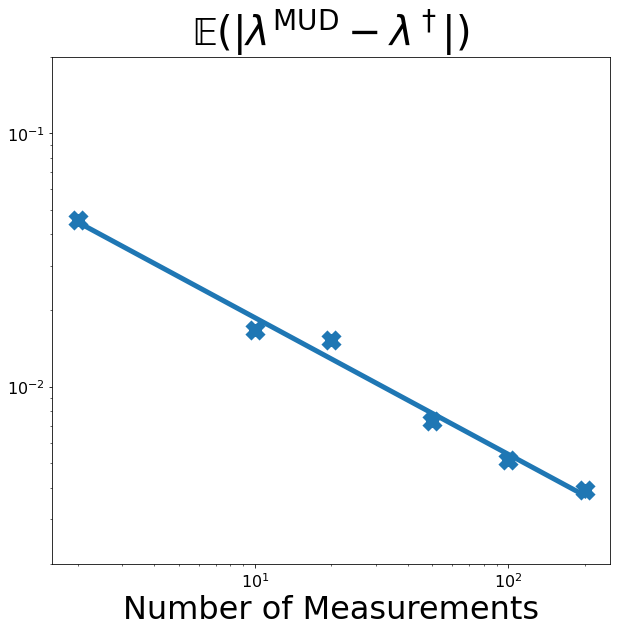
\includegraphics[width=0.45\linewidth]{figures/ode/ode_convergence_mud_obs_mean.png}
			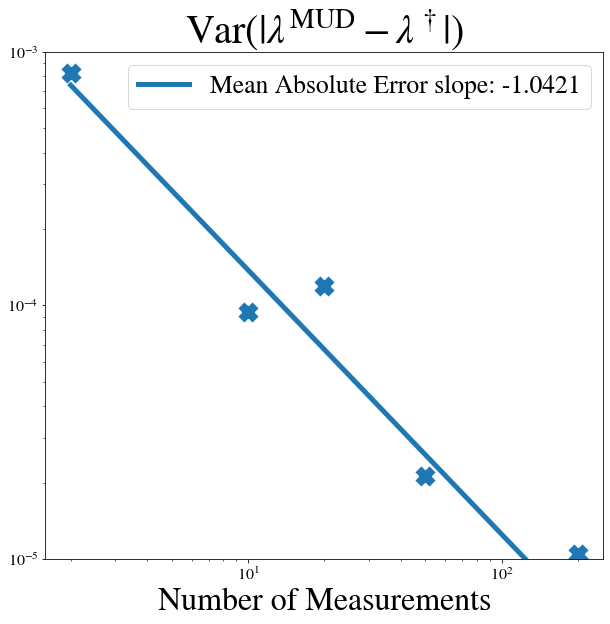
\includegraphics[width=0.45\linewidth]{figures/ode/ode_convergence_mud_obs_var.png}
	}
 %  \caption{Curves for exponential decay model with various decay coefficients. Dashed curves denote 99\% probability intervals for noise. The true signal is shown in solid black.
 % Curves associated with the MUD estimates for the decay coefficient computed from 20 trials are shown in light red.
 % Both sets of these curves encompass the true signal for $N=20$ (top plot) and $N=200$ (bottom plot) data points.
 % The light red curves are almost indistinguishable in the bottom plot as they all lie nearly on the true signal which demonstrates the overall reduction in variance in MUD estimates around the true signal when using $N=200$ data points.
 %  }
  \label{fig:ode-reference}
\end{figure}
}

\only<2>{
\begin{figure}[htb]
	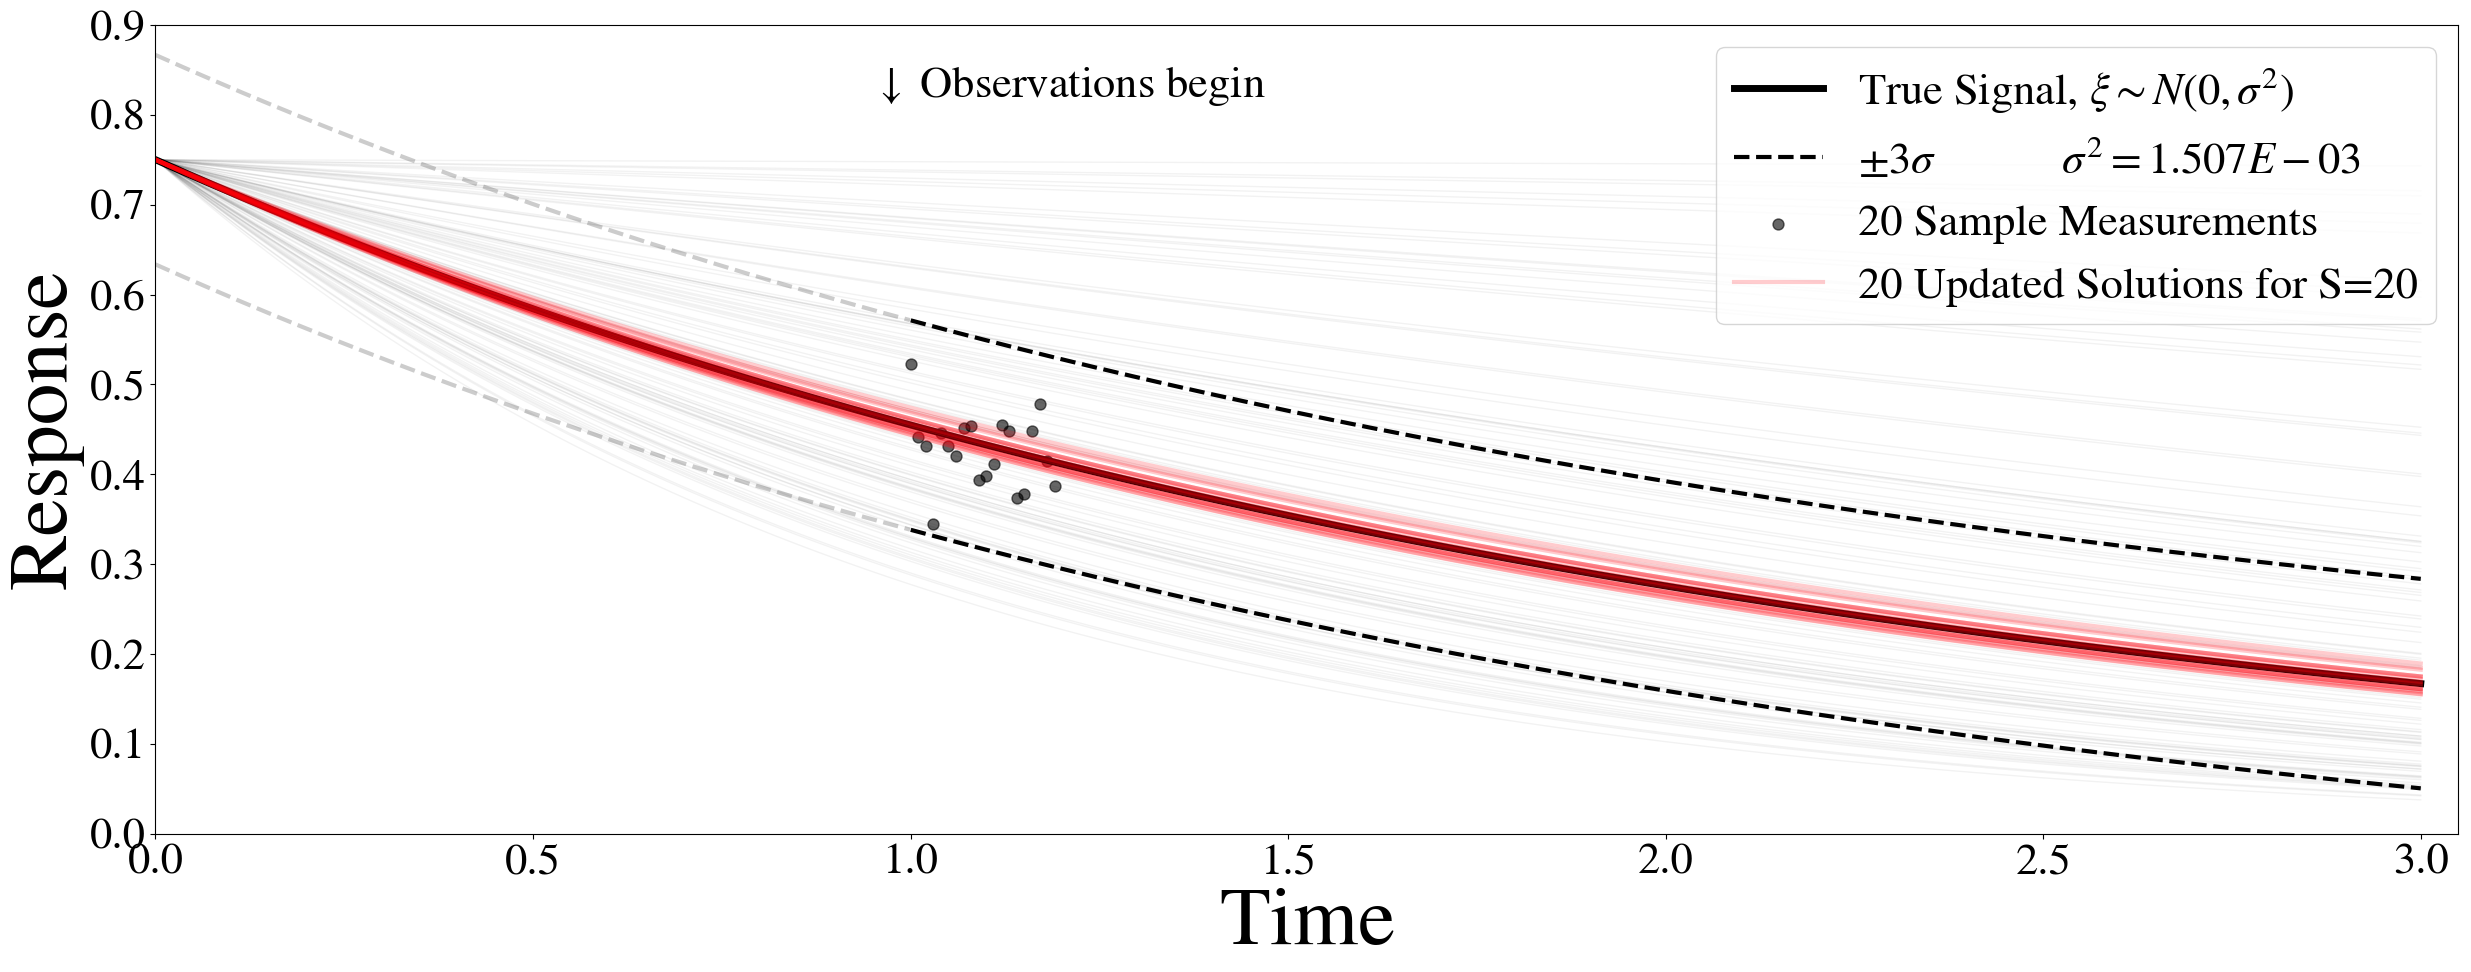
\includegraphics[width=0.85\linewidth]{figures/ode/ode_20_reference_solution.png}
	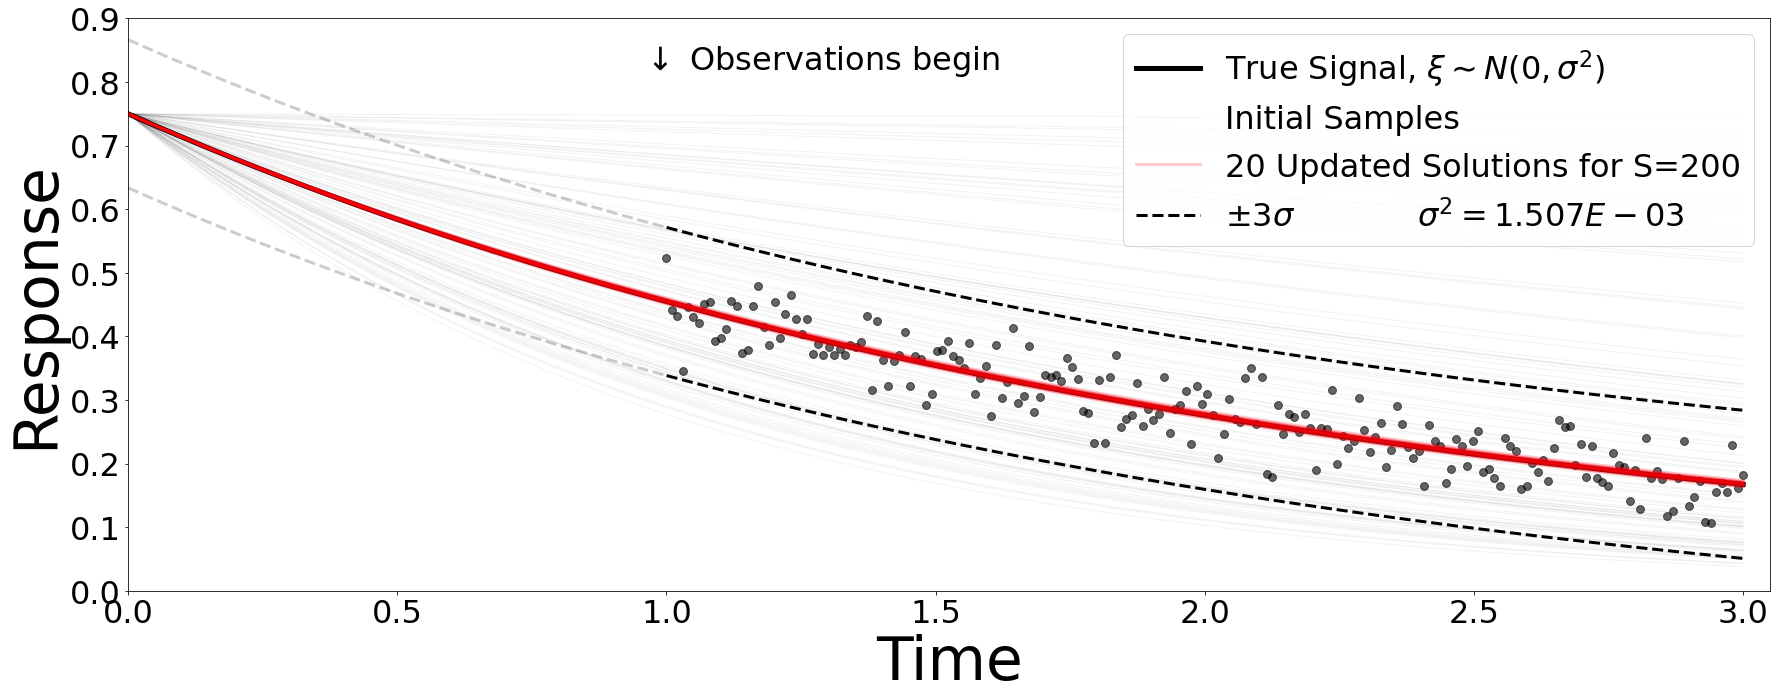
\includegraphics[width=0.85\linewidth]{figures/ode/ode_200_reference_solution.png}
  % \caption{The mean (left) and variance (right) of absolute errors in MUD estimates as a function of the number of data points used. These statistics are computed over 20 trials.
  % }
  \label{fig:ode-convergence}
\end{figure}
}

\end{frame}


%%%%%%%%%%%%%%%%%%%%%%%%%%%%%%%%%%%%%%%%%%%%%%%%%%%%%%%%%%%
\begin{frame}{\it The one where we violate some assumptions (and see what happens).}

Consider the Poisson problem:
\begin{equation}\label{eq:pde-equation}
\begin{cases}
\hfill -\nabla \cdot \nabla u &= f(x), \quad\text{on } x\in \Omega, \\
\hfill u &= 0, \quad\text{ on } \Gamma_T \cup \Gamma_B, \\
\hfill \frac{\partial u}{\partial \mathbf{n}} &= g(x_2), \quad\text{ on } \Gamma_L, \\
\hfill \frac{\partial u}{\partial \mathbf{n}} &= 0, \quad\text{ on } \Gamma_R,
\end{cases}
\end{equation}
where $x=(x_1, x_2) \in \Omega = (0,1)^2$ is the spatial domain.

\bigskip
\begin{itemize}
\item $\Gamma_T$, $\Gamma_B$, $\Gamma_L$, and $\Gamma_R$, denote the top, bottom, left, and right boundaries.
\bigskip
\item The outward normal derivative is denoted by $\frac{\partial u}{\partial \mathbf{n}}$.
\bigskip
\item The forcing function is $f = 10\exp\left ( \norm{x - 0.5}^2 / 0.02 \right )$.
\end{itemize}

\end{frame}


%%%%%%%%%%%%%%%%%%%%%%%%%%%%%%%%%%%%%%%%%%%%%%%%%%%%%%%%%%%
\begin{frame}[t]

\begin{itemize}

\item $g(x_2)$ is uncertain parameter, i.e., $\param$ defines an uncertain function.

\bigskip
\item To generate the noisy data, we use $g(x_2)\propto x_2^2(x_2-1)^5$.

\bigskip
\item Constant of proportionality chosen so $\min{g}=-3$ at $x_2=\frac{2}{7}$.

\bigskip
\bigskip
\item Piecewise-linear finite elements on a triangulation of a $36\times36$ mesh.

\bigskip
\item 100 randomly placed sensors in the subdomain $(0.05, 0.95)^2 \subset \Omega$.

\bigskip
\bigskip
\item Repeated $20$ times to study variation due to realizations of noisy data.

\bigskip
\item Limited to $\nsamps = 1000$ samples from initial density.
\end{itemize}

\end{frame}


%%%%%%%%%%%%%%%%%%%%%%%%%%%%%%%%%%%%%%%%%%%%%%%%%%%%%%%%%%%
\begin{frame}
\begin{figure}
\centering
    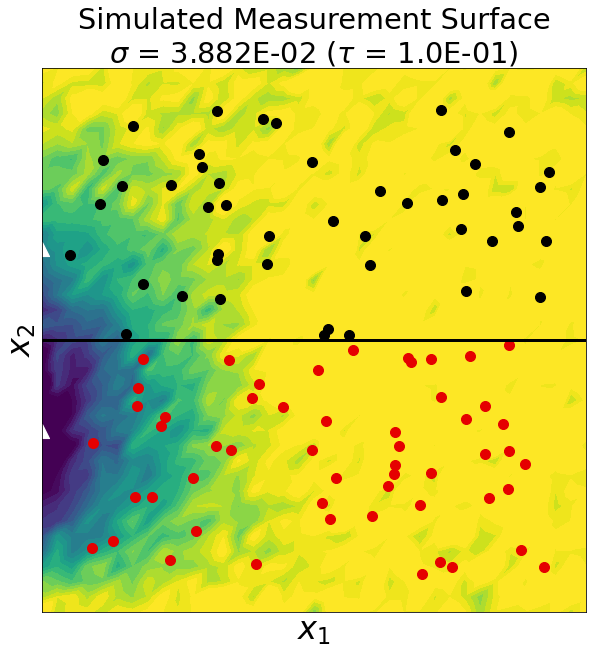
\includegraphics[width=0.5\linewidth]{figures/pde-highd/pde-highd_sensors_D2.png}
% \caption{
% A representative noisy perturbation of the reference response surface. Locations of the randomly chosen spatial data used to construct both $Q_{1D}$ and $Q_{2D}$ are shown as black and red dots.
% }
\label{fig:pde-Q}
\end{figure}
\end{frame}


%%%%%%%%%%%%%%%%%%%%%%%%%%%%%%%%%%%%%%%%%%%%%%%%%%%%%%%%%%%
\begin{frame}
\begin{figure}
\centering
    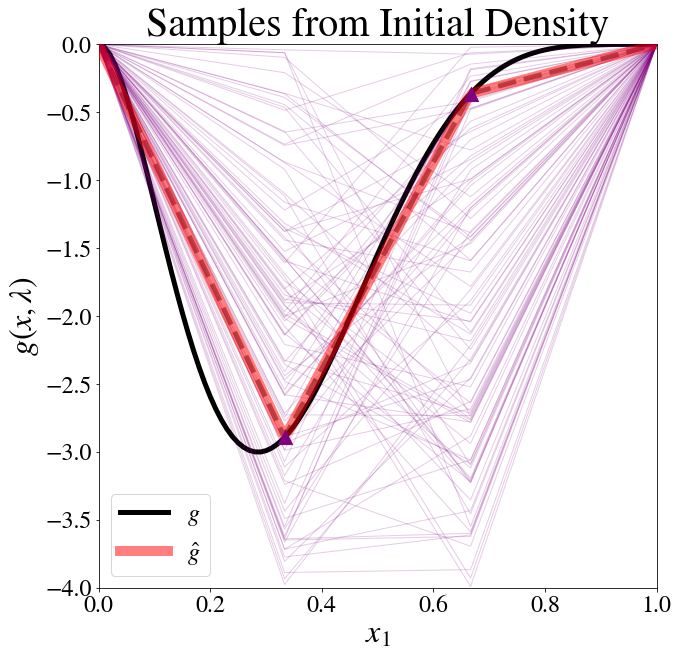
\includegraphics[width=0.325\linewidth]{figures/pde-highd/pde-highd_init_D2.png}
    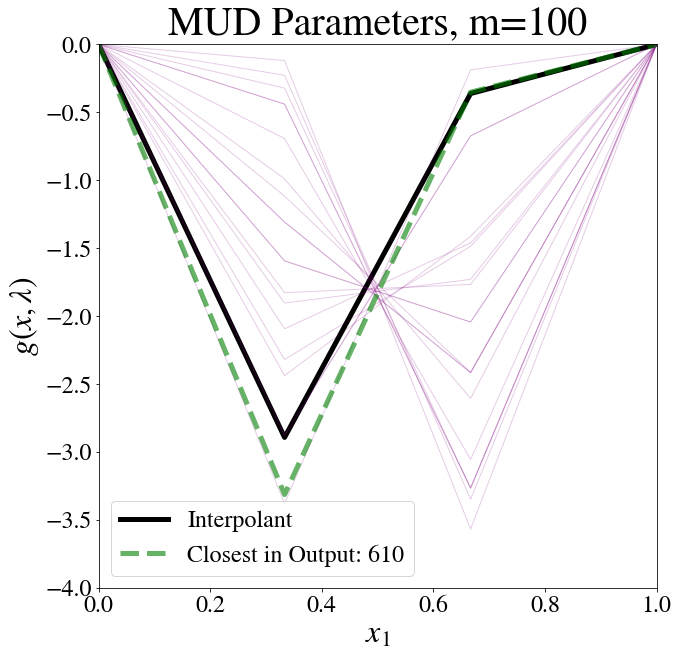
\includegraphics[width=0.325\linewidth]{figures/pde-highd/pde-highd_pair_D2-1_m100.png}
    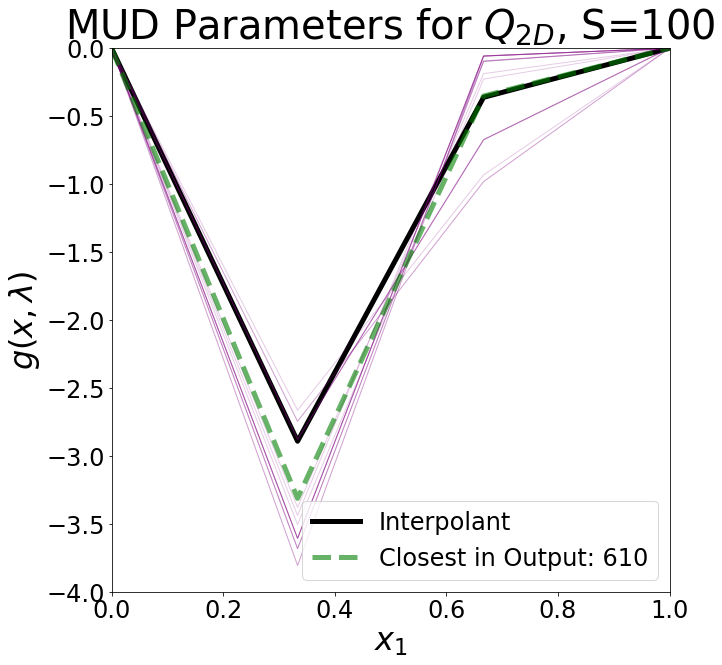
\includegraphics[width=0.325\linewidth]{figures/pde-highd/pde-highd_pair_D2-2_m100.png}
% \caption{
% In the left plot, the reference $g(x_2)$ is shown as the solid black curve with its interpolant onto the spline basis shown as a dotted red curve.
% The dashed blue line represents the sample from parameter space which most closely predicts noiseless data, which we refer to as the projection of $g$.
% The purple curves in the center and right plots show the variability in MUD estimates of $g(x_2)$ for the 20 different realizations of noisy data.
% The center plot uses $Q_{1D}$ and the right plot uses $Q_{2D}$ to construct the MUD estimates.
% }
\label{fig:pde-MUD}
\end{figure}
\end{frame}
